\documentclass[12pt,a4paper]{article}
\usepackage[utf8]{inputenc}
\usepackage{polski}
\usepackage{graphicx}
\usepackage{minted}
\usepackage{caption}
\usepackage{url}
\usepackage{framed}
\usepackage[normalem]{ulem}
\usepackage{amsmath}
\usepackage{amsthm}
\usepackage{amssymb}
\usepackage{amsfonts}
\usepackage{enumerate}
\usepackage{booktabs}
\usepackage[utf8]{inputenc}
\usepackage[table,xcdraw,usenames,dvipsnames,svgnames]{xcolor}
\usepackage[left=2.5cm, right=2.5cm, top=3.0cm, bottom=3.0cm]{geometry}

%A bunch of definitions that make my life easier
\newcommand{\matlab}{{\sc Matlab} }
\newcommand{\cvec}[1]{{\mathbf #1}}
\newcommand{\rvec}[1]{\vec{\mathbf #1}}
\newcommand{\ihat}{\hat{\textbf{\i}}}
\newcommand{\jhat}{\hat{\textbf{\j}}}
\newcommand{\khat}{\hat{\textbf{k}}}
\newcommand{\minor}{{\rm minor}}
\newcommand{\trace}{{\rm trace}}
\newcommand{\spn}{{\rm Span}}
\newcommand{\rem}{{\rm rem}}
\newcommand{\ran}{{\rm range}}
\newcommand{\range}{{\rm range}}
\newcommand{\mdiv}{{\rm div}}
\newcommand{\proj}{{\rm proj}}
\newcommand{\R}{\mathbb{R}}
\newcommand{\N}{\mathbb{N}}
\newcommand{\Q}{\mathbb{Q}}
\newcommand{\Z}{\mathbb{Z}}
\newcommand{\<}{\langle}
\renewcommand{\>}{\rangle}
\renewcommand{\emptyset}{\varnothing}
\newcommand{\attn}[1]{\textbf{#1}}
\theoremstyle{definition}
\newtheorem{theorem}{Theorem}
\newtheorem{corollary}{Corollary}
\newtheorem*{definition}{Definition}
\newtheorem*{example}{Example}
\newtheorem*{note}{Note}
\newtheorem{exercise}{Exercise}
\newcommand{\bproof}{\bigskip {\bf Proof. }}
\newcommand{\eproof}{\hfill\qedsymbol}
\newcommand{\Disp}{\displaystyle}
\newcommand{\qe}{\hfill\(\bigtriangledown\)}
\renewcommand\refname{Żródła}
\setlength{\columnseprule}{1 pt}
\linespread{1.5}

\setminted{
    linenos=true,
    autogobble,
    breaklines,
    frame=lines,
    framerule=1pt,
    framesep=9pt,
    fontsize=\small
}

\setlength{\abovecaptionskip}{0pt}
\setlength\parskip{1em}

\setlength\parindent{0pt} % no indentation of paragraphs
%\usepackage{indentfirst} % indent all paragraphs (the ones following section headers as well

\newenvironment{longlisting}{\captionsetup{type=listing}}{}
\renewcommand\listingscaption{Code}
 
\DeclareCaptionType{myequation}[][Równanie parametryczne]
%\captionsetup[myequation]{labelformat=empty}

\makeatletter
\newcommand{\linia}{\rule{\linewidth}{0.4mm}}
\renewcommand{\maketitle}{\begin{titlepage}
    \vspace*{1cm}
    \begin{center}\small
    Politechnika Wrocławska\\
    Wydział Elektroniki
    \end{center}
    \vspace{3cm}
    \noindent\linia
    \begin{center}
      \LARGE \textsc{\@title}
         \end{center}
     \linia
    \vspace{0.5cm}
    \begin{flushright}
    \begin{minipage}{7cm}
    \textit{\small Autorzy:}\\
    \normalsize \textsc{\@author} \par
    \end{minipage}
    \vspace{5cm}

     {}
     \end{flushright}
    \vspace*{\stretch{6}}
    \begin{center}
    \@date
    \end{center}
  \end{titlepage}%
}
\makeatother
\author{Dariusz Tomaszewski, 235565\newline Bartosz Rodziewicz, 226105}
\title{technonogie chmury obliczeniowej i~centrum danych\\
\normalsize{temat projektu: domowe centrum multimedialne}}

\begin{document}
\maketitle
\tableofcontents
\newpage

\section{Założenia projektowe}

Projekt polega na utworzeniu domowego serwera multimedialnego z kilkoma dyskami działającymi w RAID na których mogą być składowane multimedia domowe (zdjęcia, muzyka, filmy). Zarządzanie multimediami dostępnymi na serwerze ma być dostępne w przeglądarce za pomocą interfejsu jaki można spotkać w popularnych rozwiązaniach chmurowych do przechowywania danych. Należy również zapewnić możliwość strumieniowania multimediów na urządzenia Smart z wykorzystaniem protokołu DLNA.

\section{Koncepcja rozwiązania}

Serwer zostanie oparty o oprogramowanie TrueNAS, które daje użytkownikom i urządzeniom klienckim dostęp do współdzielonych danych za pośrednictwem praktycznie dowolnego protokołu udostępniania dzięki możliwości instalacji pluginów, które rozszerzają możliwości systemu TrueNAS o dowolne funkcjonalności.

Interfejs przeglądarkowy dla plików zostanie zrealizowany za pomocą nextCloud, który jest forkiem słabiej już rozwijanego OwnCloud. Podstawowym zadaniem Nextcloud jest dostęp do plików z każdego miejsca, zarówno na urządzeniach stacjonarnych, jak i mobilnych. Możliwy jest dostęp przez stronę Web, a także za pomocą aplikacji dla systemów Android i iOS. Chmura pozwala przesyłać pliki, współdzielić je z innymi użytkownikami oraz otrzymywać powiadomienia gdy ktoś udostępni dane. Pliki oznaczone są regułami i parametrami, takimi jak fizyczna lokalizacja, grupa użytkowników, właściwości plików, typy plików. Wskazane parametry pozwalają administratorom w pełni kontrolować dostęp do danych.

Filmy wykorzystane w przykładach działania pochodzą ze strony \url{www.pexels.com} i są one na licencji Creative Commons.

\section{Implementacja rozwiązania}
\subsection{Instalacja TrueNAS}

Do instalacji TrueNAS wykorzystaliśmy maszynę wirtualną oferowaną przez oprogramowanie VirtualBox. Parametry maszyny wirtualnej jakie ustawiliśmy widoczne są na Rysunku~\ref{vb_settings}.

\begin{figure}[H]
    \centering
    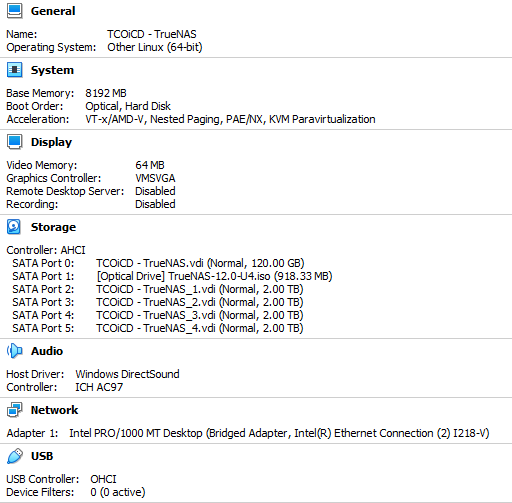
\includegraphics[width=\linewidth]{img/ss_truenas/1.png}
    \caption{Ustawienia maszyny wirtualnej}
    \label{vb_settings}
\end{figure}

Następnie zamontowaliśmy obraz ISO oprogramowania TrueNAS CORE w wersji 12.0-U4, który został pobrany ze strony producenta. Po uruchomieniu maszyny wirtualnej otrzymaliśmy menu wyboru widoczne na Rysunku~\ref{grub} w którym wybraliśmy opcję 1.

\begin{figure}[H]
    \centering
    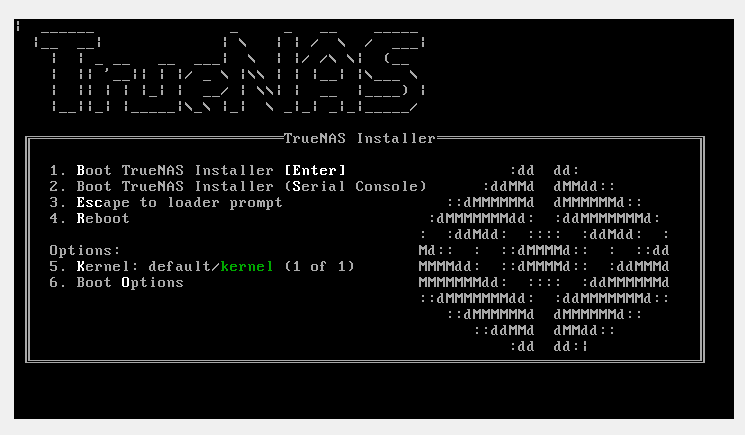
\includegraphics[width=14cm]{img/ss_truenas/2.png}
    \caption{Menu wyboru GRUB}
    \label{grub}
\end{figure}

Na następnym ekranie widzimy menu instalacyjne, które pyta jaką akcję chcemy wykonać. Chcemy zainstalować TrueNAS, więc wybieramy opcję 1.

\begin{figure}[H]
    \centering
    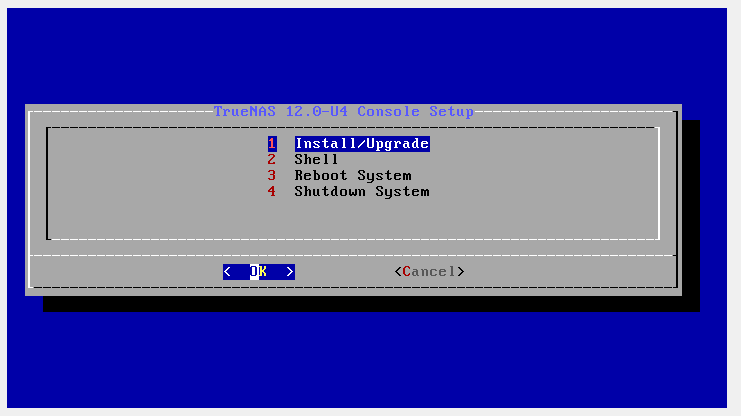
\includegraphics[width=\linewidth]{img/ss_truenas/3.png}
    \caption{Menu instalacji TrueNAS}
    \label{install_menu}
\end{figure}

Następnie instalator pyta nas na którym dysku chcemy zainstalować system. Wybieramy odpowiedni dysk i zatwierdzamy wybór. W stworzonej przez nasz maszynie emulujemy jeden dysk SSD 120GiB oraz 4 dyski HDD o rozmiarze 2TiB każdy. Z wiadomych względów system TrueNas zostaje zainstalowany na dysku SSD.

\begin{figure}[H]
    \centering
    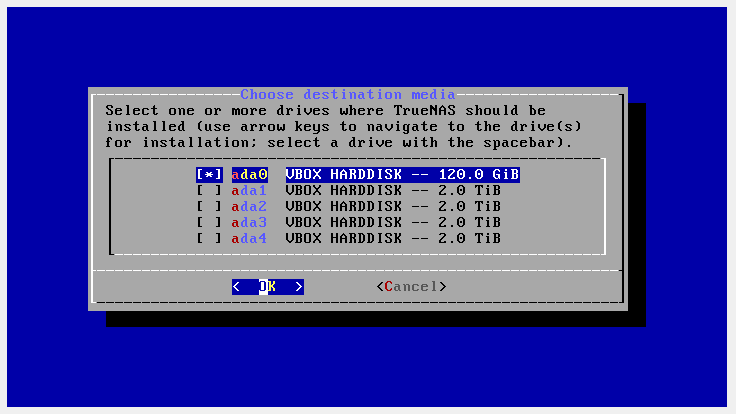
\includegraphics[width=\linewidth]{img/ss_truenas/4.png}
    \caption{Menu wyboru dysku do instalacji}
    \label{install_disk_menu}
\end{figure}

Otrzymujemy ostrzeżenie, że wszystkie dane na wybranym dysku zostaną wymazane oraz że nie będzie można używać tego dysku do udostępniania danych. Zatwierdzamy.

\begin{figure}[H]
    \centering
    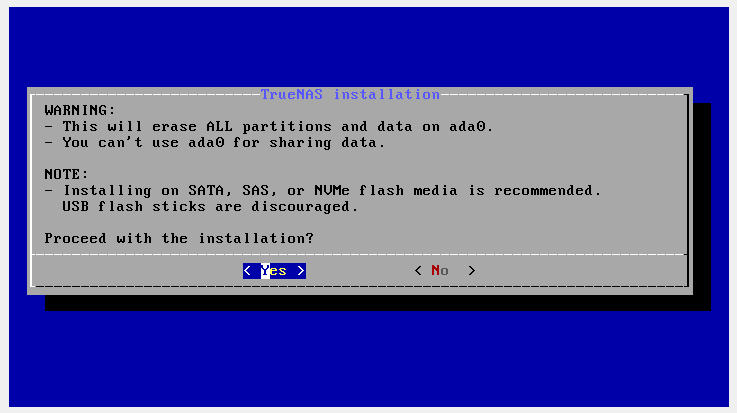
\includegraphics[width=\linewidth]{img/ss_truenas/5.png}
    \caption{Ostrzeżenie o usunięciu danych z dysku instalacji}
    \label{install_data_warning}
\end{figure}

Na następnym ekranie instalator pyta nas jakie chcemy ustawić hasło dla użytkownika $root$. Dla pewności, że wszystko będzie działać poprawnie, ustawiamy hasło $x$ i zatwierdzamy. Oczywiście w prawdziwym setupie ustawione tutaj hasło powinno być długie i bezpieczne, ponieważ chroni ono dostęp do zarządzania całym serwerem NAS. Dodatkowo zalecane jest włączenie 2FA, co możliwe jest później po instalacji systemu w panelu zarządzania.

\begin{figure}[H]
    \centering
    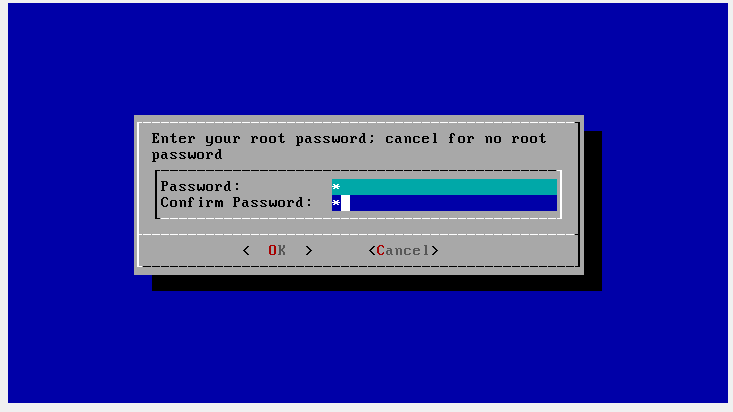
\includegraphics[width=\linewidth]{img/ss_truenas/6.png}
    \caption{Ustawianie hasła użytkownika root}
    \label{set_password_root}
\end{figure}

Instalator pyta nas również o tryb bootowania. Wybieramy opcję UEFI ze względu na to, że jest to nowsze rozwiązanie i takie też zastosowaliśmy ustawienie dla maszyny wirtualnej.

\begin{figure}[H]
    \centering
    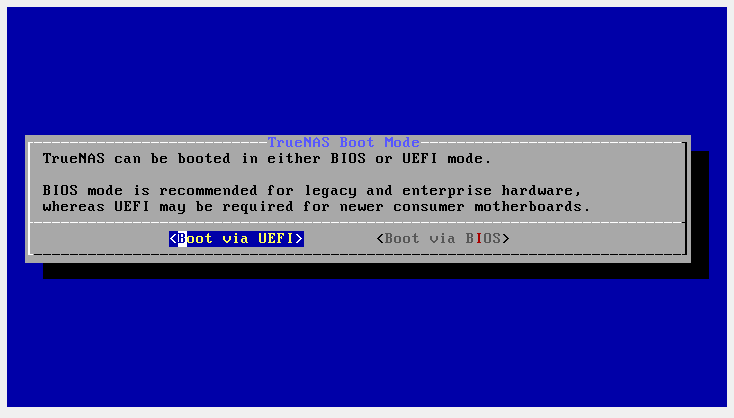
\includegraphics[width=\linewidth]{img/ss_truenas/7.png}
    \caption{Wybór $Boot Mode$}
    \label{install_uefi}
\end{figure}

Tworzymy również partycję SWAP.
\begin{figure}[H]
    \centering
    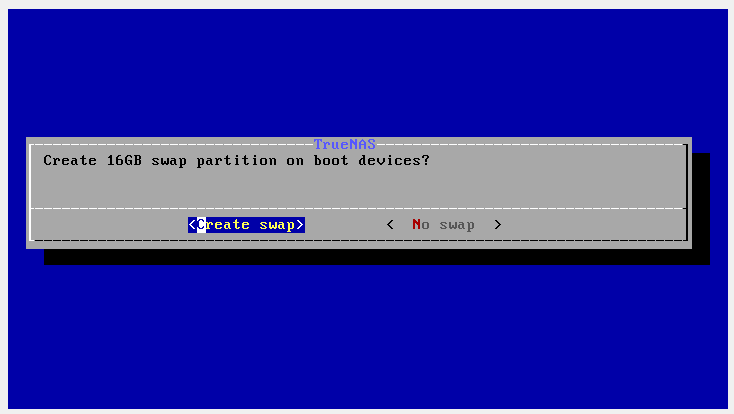
\includegraphics[width=\linewidth]{img/ss_truenas/8.png}
    \caption{Tworzenie partycji SWAP}
    \label{install_swap}
\end{figure}

W tym momencie rozpoczyna się instalacja TrueNAS. po zakończonej instalacji zobaczymy taki komunikat:

\begin{figure}[H]
    \centering
    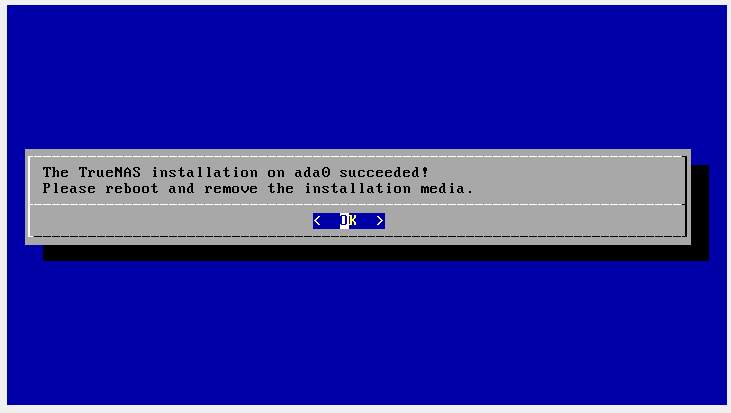
\includegraphics[width=\linewidth]{img/ss_truenas/11.png}
    \caption{Zakończona instalacja}
    \label{install_complete}
\end{figure}


Możemy już odłączyć nośnik z instalatorem i zrestartować maszynę. Po restarcie uruchamiamy TrueNAS, który po uruchomieniu przywita nas ekranem z menu wyboru oraz co jest ważne, linkami do interfejsu webowego. Od tej pory wszelka konfiguracja będzie odbywała się z poziomu interfejsu webowego.

\begin{figure}[H]
    \centering
    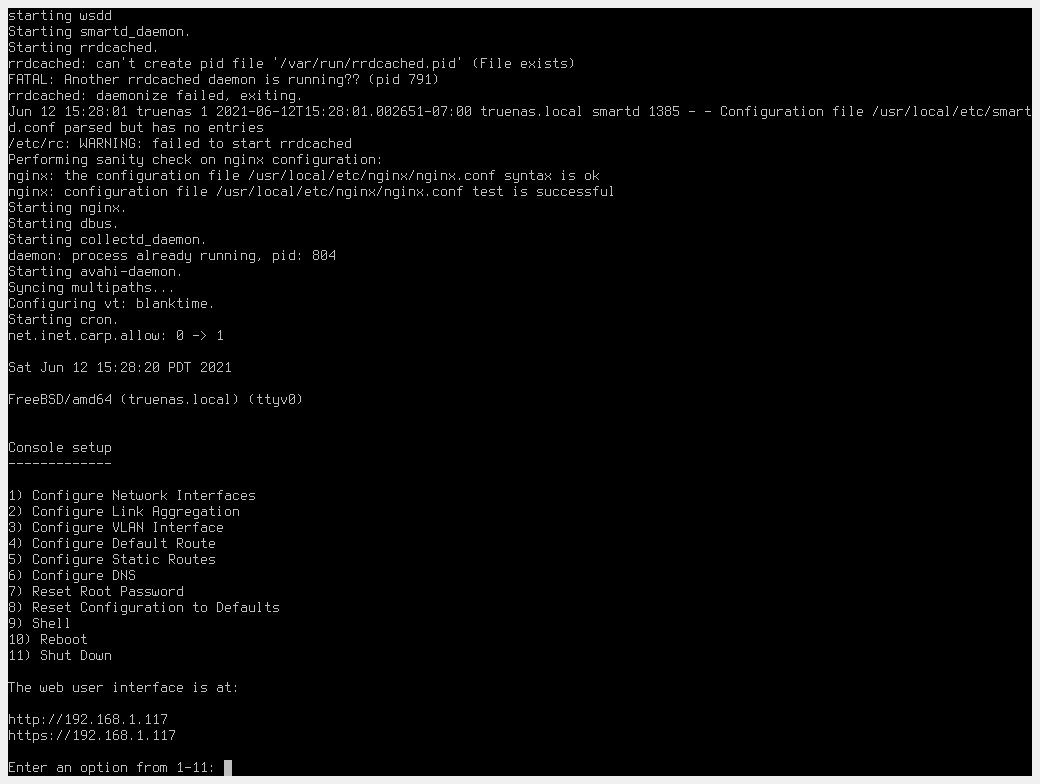
\includegraphics[width=\linewidth]{img/ss_truenas/14.png}
    \caption{Konsola TrueNAS z adresami do interfejsu webowego}
    \label{vm_cli}
\end{figure}

\newpage
\subsection{Konfiguracja TrueNAS}

Po wejściu na adres pod którym skonfigurowana jest maszyna wirtualna, zobaczymy ekran logowania. Podajemy tutaj dane logowania dla użytkownika $root$, w tym hasło, które ustawiliśmy podczas instalacji.

\begin{figure}[H]
    \centering
    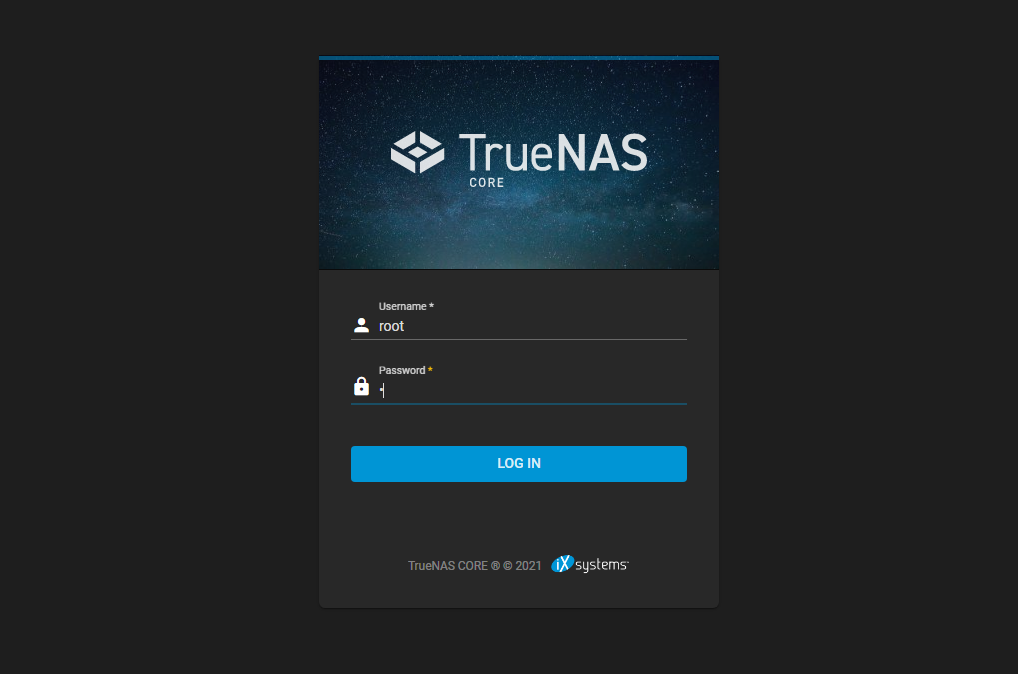
\includegraphics[width=\linewidth]{img/ss_truenas/16.png}
    \caption{Panel logowania}
    \label{login_screen}
\end{figure}

Po zalogowaniu uzyskujemy dostęp do interfejsu sieciowego TrueNAS, który służy do zarządzania dyskami, konfigurowania dostępu do przechowywanych danych oraz przeglądania stanu systemu.

\begin{figure}[H]
    \centering
    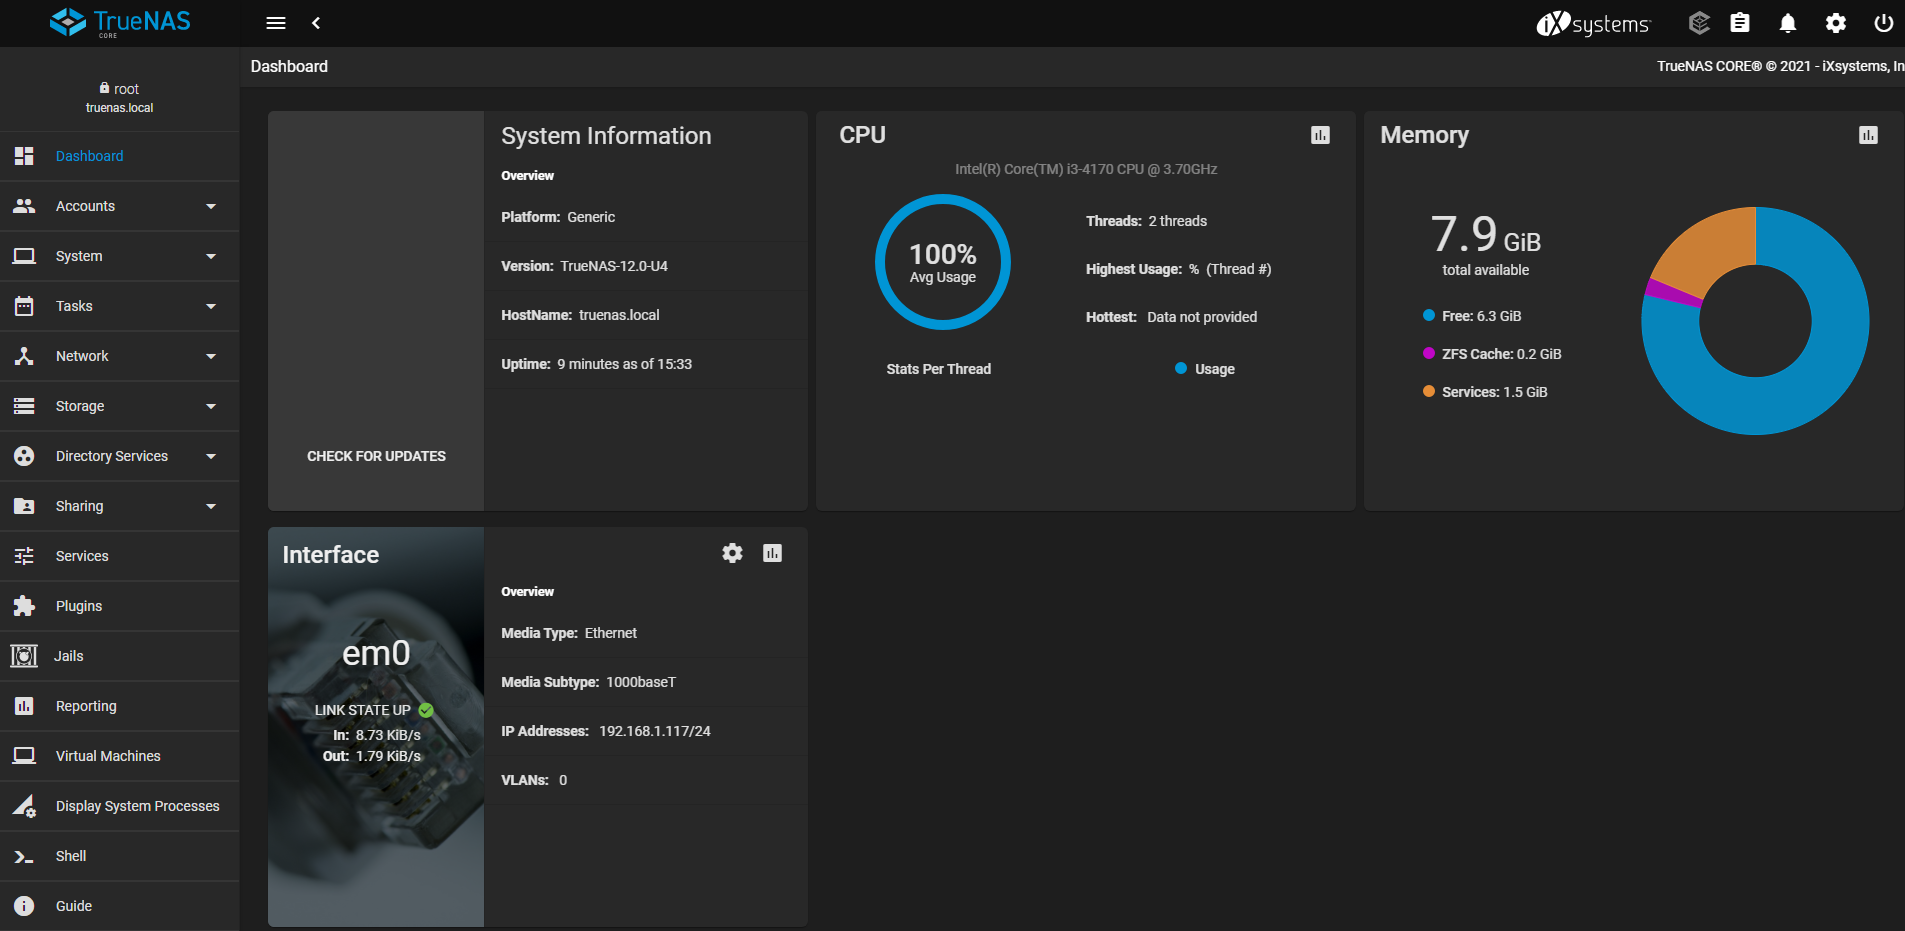
\includegraphics[width=\linewidth]{img/ss_truenas/17.png}
    \caption{Dashboard}
    \label{dashboard}
\end{figure}

Część storage'owa jest najważniejsza w serwerach NAS, więc na początku ją konfigurujemy.

Tworzenie nowego datapoolu odbywa się w zakładce Storage Pools. Tworząc nowy pool uruchamia nam się menadżer pooli, gdzie ustawiamy nazwę, dyski wchodzące w skład poola oraz typ RAID.

\begin{figure}[H]
    \centering
    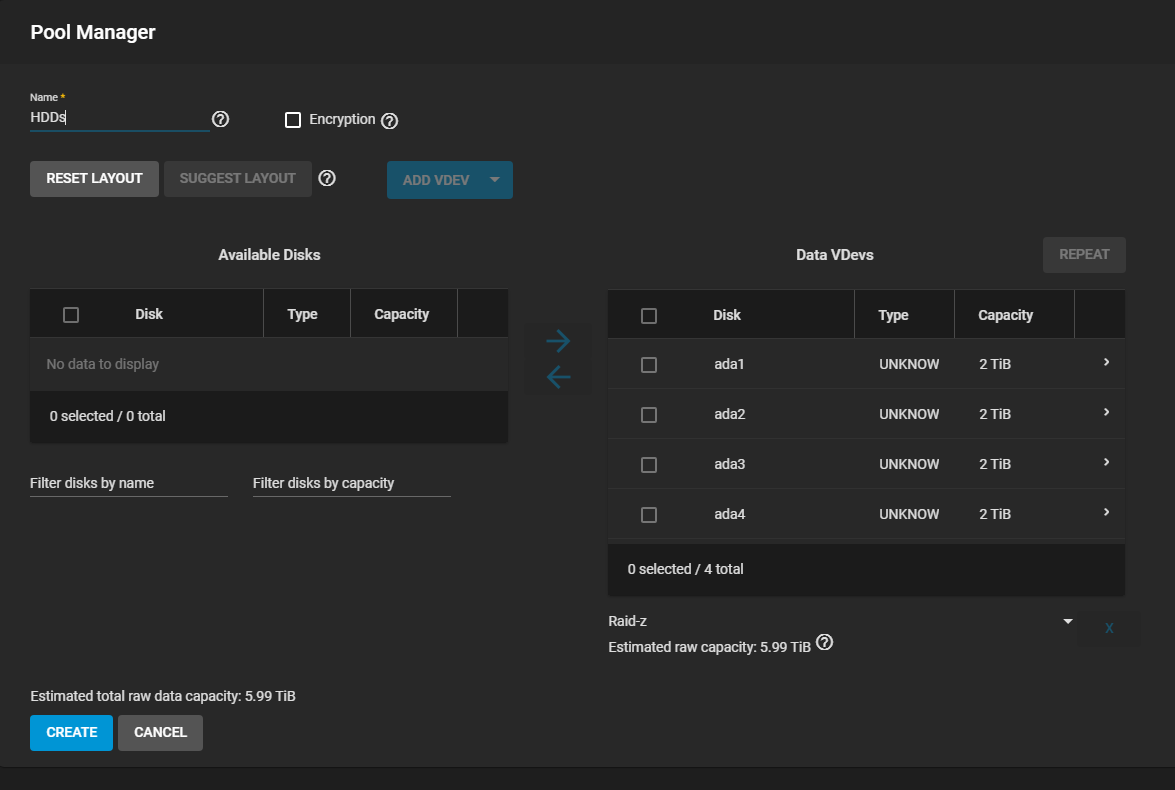
\includegraphics[width=\linewidth]{img/ss_truenas/20.png}
    \caption{Widok tworzenia poola}
    \label{pool_manager}
\end{figure}

W TrueNAS mamy dostępne następujące RAIDy:
\begin{itemize}
    \item $Stripe$ - odpowiednik RAID0
    \item $Mirror$ - odpowiednik RAID1
    \item $Raid-z$ - odpowiednik RAID5
    \item $Raid-z2$ - odpowiednik RAID6
    \item $Raid-z3$, $z4$, ... - cyfra po literze z oznacza ile dysków może ulec uszkodzeniu bez utraty danych
\end{itemize}

W przypadku dostępnych 4 dysków RAID5 wydaje się najrozsądniejszym rozwiązaniem. Warto tutaj postarać się by dyski do naszego NASa nie pochodziły z tej samej partii by zminimalizować ryzyko awarii kilku dysków w podobnym czasie (np. kupować dyski od różnych sprzedawców).

\begin{figure}[H]
    \centering
    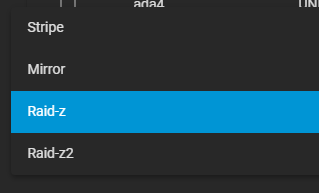
\includegraphics{img/ss_truenas/21.png}
    \caption{Wybór $Raid-z$}
    \label{pool_raidz}
\end{figure}

W tym momencie TrueNAS tworzy poola. Po utworzeniu poola pojawi się on na liście pooli, która pokazuje również ich najważniejsze parametry.

\begin{figure}[H]
    \centering
    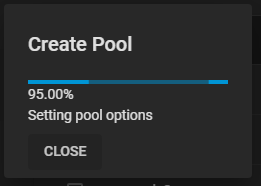
\includegraphics{img/ss_truenas/24.png}
    \caption{Proces tworzenia Pool'a}
    \label{pool_creating_progress}
\end{figure}

Oprócz poola należy również utworzyć dataset. Dataset jest systemem plików, który jest tworzony w ramach pooli. Datasety mogą zawierać pliki, katalogi i mieć indywidualne uprawnienia lub flagi. Datasety mogą być również szyfrowane, albo przy użyciu szyfrowania utworzonego z pooli lub z oddzielną konfiguracją szyfrowania.
Aby utworzyć dataset należy kliknąć na ustawienia danego poola i wybrać utworzenie datasetu. W naszym przypadku utworzyliśmy dataset z domyślnymi ustawieniami.

\begin{figure}[H]
    \centering
    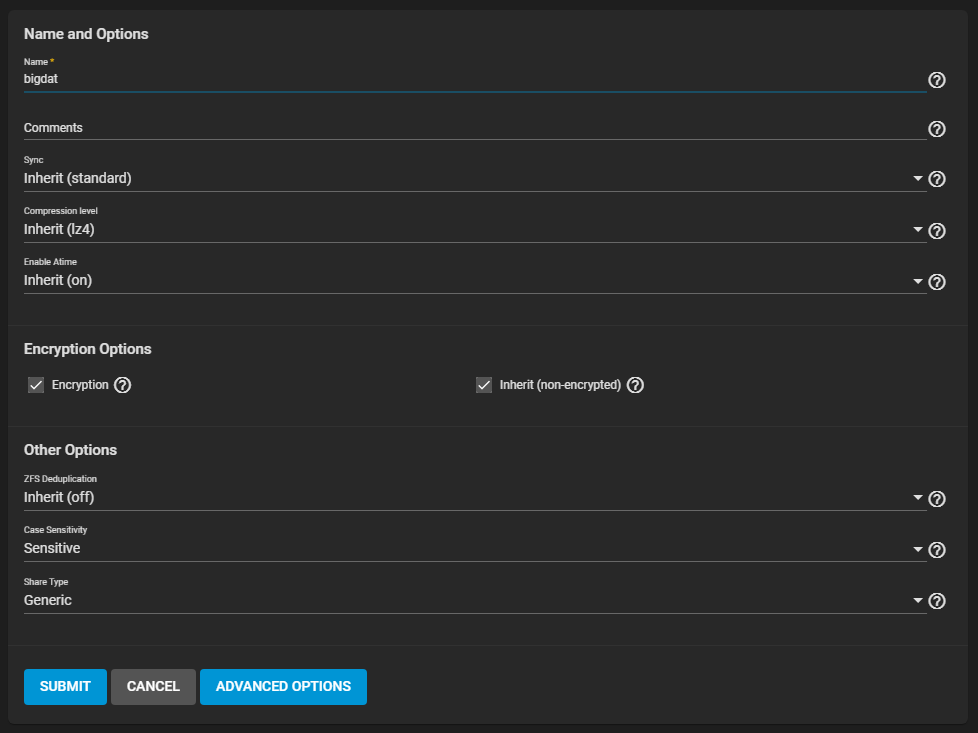
\includegraphics[width=\linewidth]{img/ss_truenas/26.png}
    \caption{Tworzenie dataseta}
    \label{dataset_creating}
\end{figure}

Po tej operacji widzimy utworzony dataset w obrębie danego poola.

\begin{figure}[H]
    \centering
    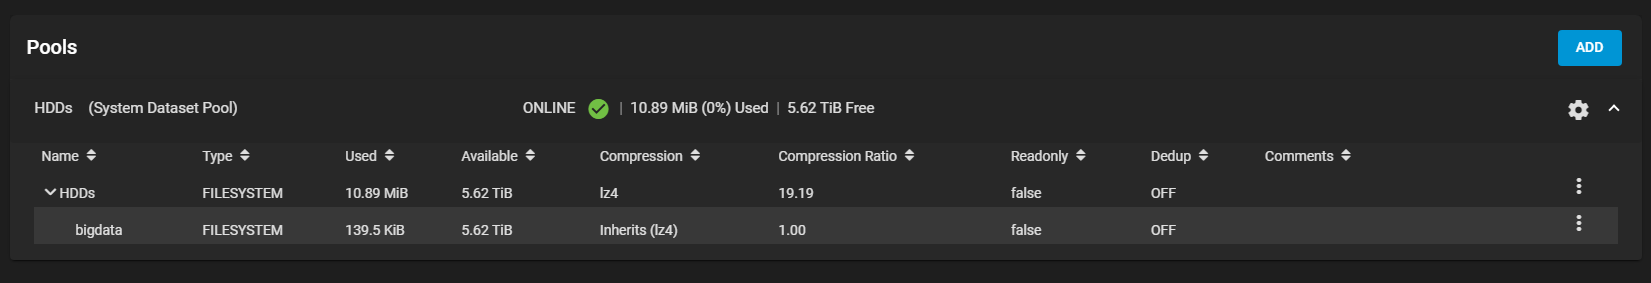
\includegraphics[width=\linewidth]{img/ss_truenas/27.png}
    \caption{Lista datapooli i setów}
    \label{pool_list_group}
\end{figure}

Następnym krokiem jest stworzenie konta użytkownika by nie logować się do zasobów kontem roota. W przypadków share'ów Windowsowych możliwe jest stworzenie konta zgodnego z nazwą i hasłem konta w systemie by nie musieć wpisywać hasła przy próbie dostępu. Aby to aktywować konieczna jest aktywacja ustawienia Microsoft Account.

\begin{figure}[H]
    \centering
    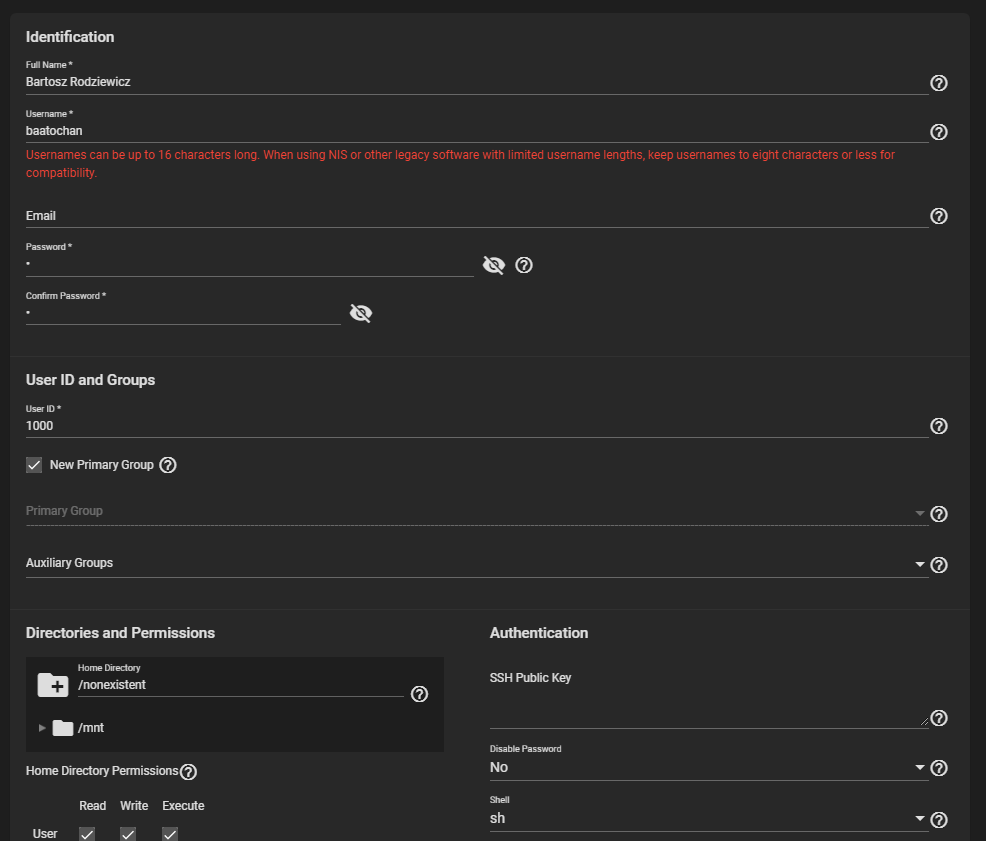
\includegraphics[width=\linewidth]{img/ss_truenas/28.png}
    \caption{Tworzenie nowego użytkownika}
\end{figure}
\begin{figure}[H]
    \centering
    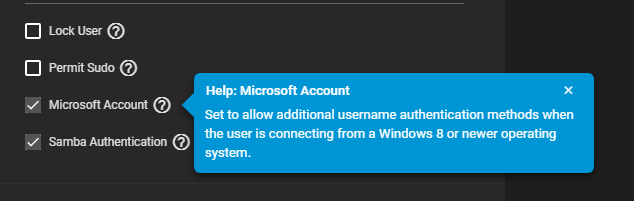
\includegraphics[width=\linewidth]{img/ss_truenas/29.png}
    \caption{Ustawienie aktywujące autologowanie pod Windowsem w przypadku zgodności username'a i hasła}
\end{figure}

Po stworzeniu użytkownika widzimy go na liście.

\begin{figure}[H]
    \centering
    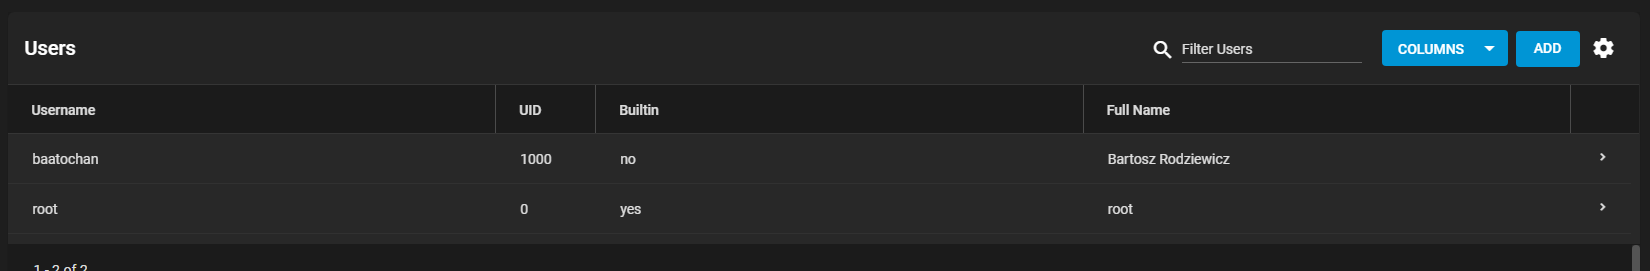
\includegraphics[width=\linewidth]{img/ss_truenas/31.png}
    \caption{Lista użytkowników}
    \label{users_list2}
\end{figure}

Po skonfigurowaniu datapoola widzimy nową kartę na dashboardzie, która pokazuje stan tego poola.

\begin{figure}[H]
    \centering
    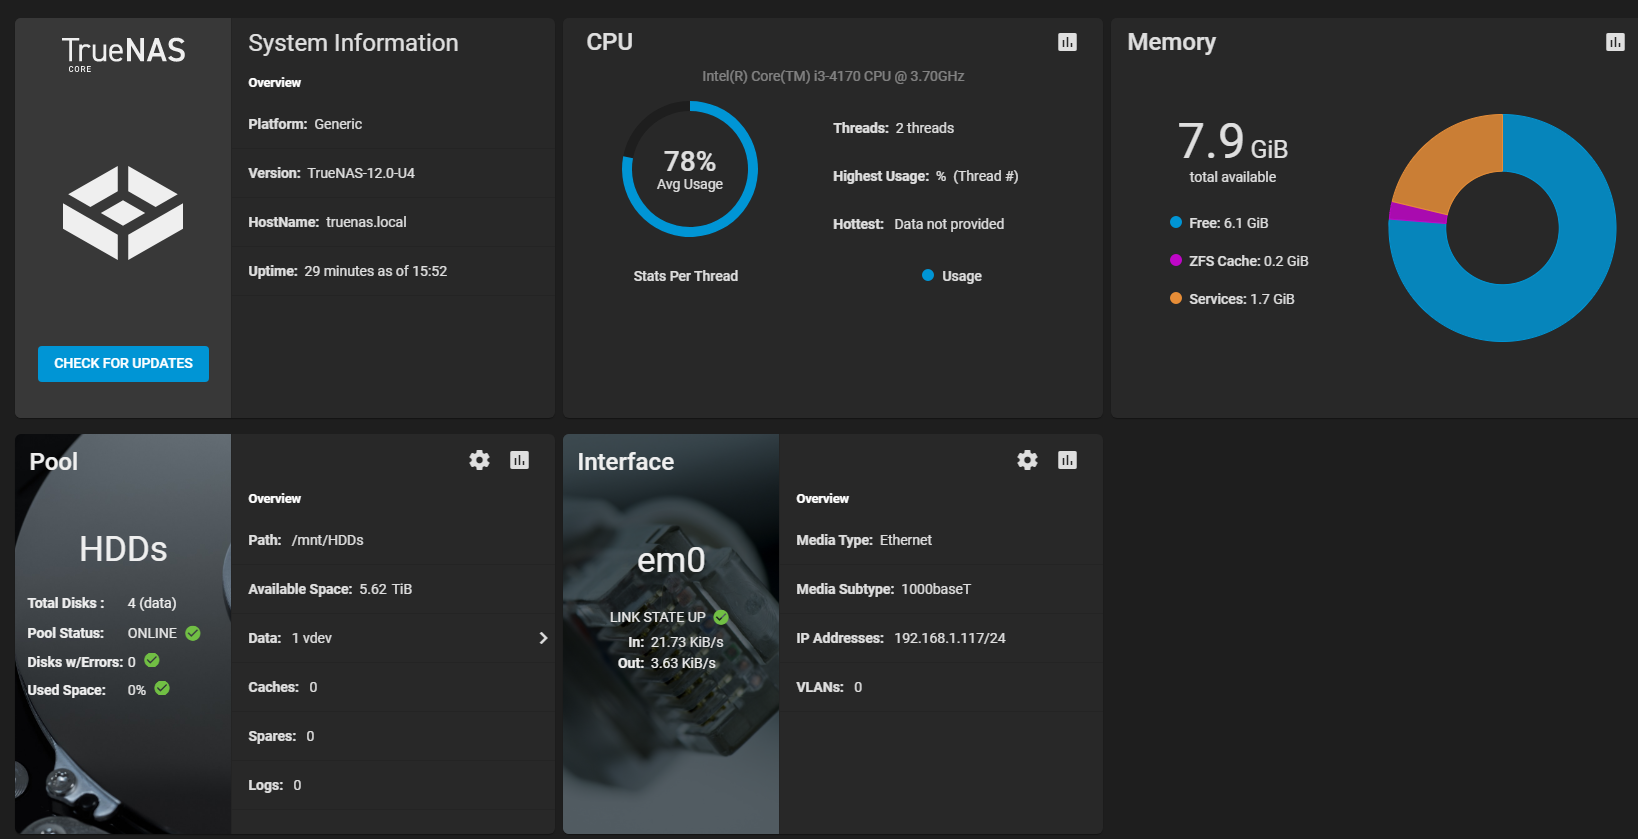
\includegraphics[width=\linewidth]{img/ss_truenas/32.png}
    \caption{Dashboard po konfiguracji Pool'a}
    \label{dashboard_after_pool}
\end{figure}

Teraz kolejnym krokiem było przejrzenie ustawień. Z głównych warto wspomnieć aktywację dostępu do interfejsu webowego tylko po HTTPS oraz ustawienie poprawnej strefy czasowej by mieć zgodne daty w zapisywanych na NASie plikach.

\begin{figure}[H]
    \centering
    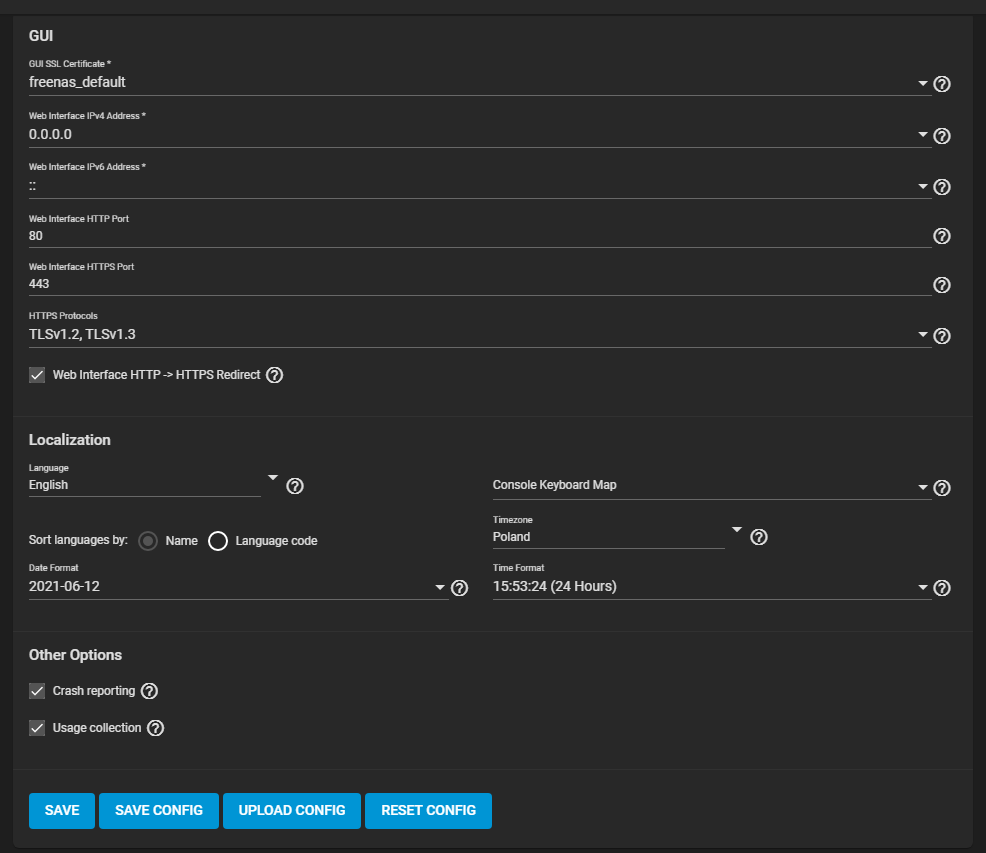
\includegraphics[width=\linewidth]{img/ss_truenas/33.png}
    \caption{Podstawowe ustawienia TrueNAS}
\end{figure}

Po aktywacji wymuszania połączenia HTTPS przeglądarka przełącza się na połączenie SSL jednak wyświetla ostrzeżenie o niezaufanym certyfikacie. Dopóki zarządzanie NASem pozostaje w sieci lokalnej nie jest to jednak bardzo istotne.

\begin{figure}[H]
    \centering
    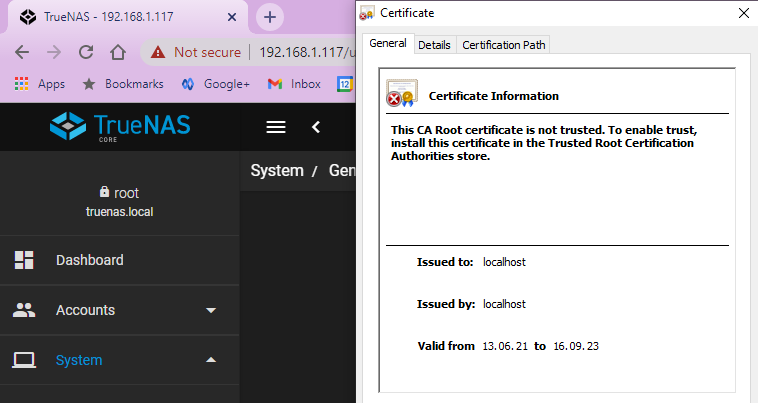
\includegraphics[width=\linewidth]{img/ss_truenas/34.png}
    \caption{Niezaufany certyfikat}
    \label{certificate}
\end{figure}

Następnym krokiem jest stworzenie Samba share'a, aby mieć dostęp do zasobów z poziomu Windowsa. Share'a przypisujemy do utworzonego przez nas dataseta.

\begin{figure}[H]
    \centering
    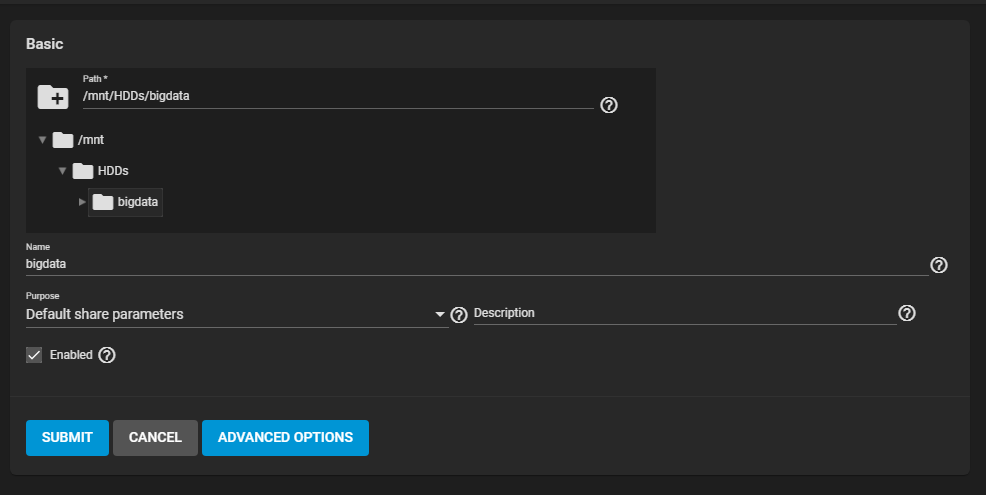
\includegraphics[width=\linewidth]{img/ss_truenas/38.png}
    \caption{Ekran tworzenia share'a}
    \label{users_list}
\end{figure}

Po stworzeniu share'a jesteśmy poinformowani o konieczności stworzenia listy ACL zabezpieczającej zasób. W tym miejscu, jako, że dostęp do share'a ma być tylko lokalny w gronie zaufanych użytkowników ustawiliśmy ACL na presecie otwartym, czyli pełną kontrolę nad plikami ma właściciel (jako, że to główny dataset to właścicielem jest root) a możliwość edycji ma każdy.

\begin{figure}[H]
    \centering
    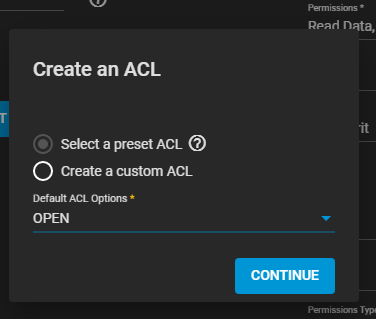
\includegraphics[width=8cm]{img/ss_truenas/41.png}
    \caption{Tworzenie ACL na podstawie presetu}
\end{figure}
\begin{figure}[H]
    \centering
    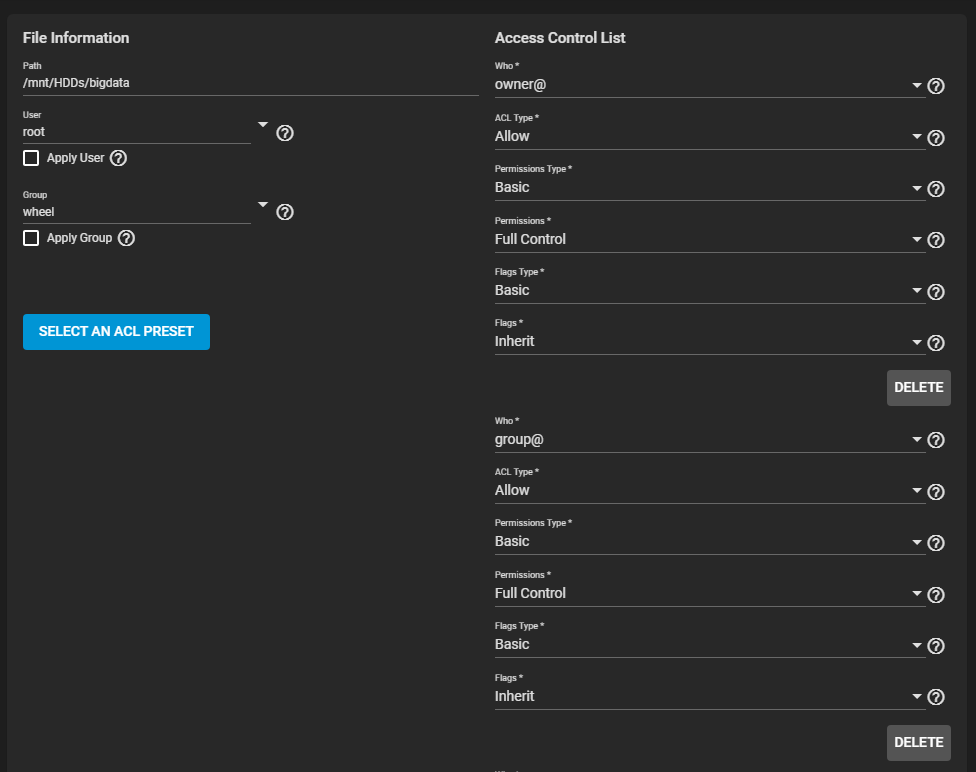
\includegraphics[width=15cm]{img/ss_truenas/42.png}
    \caption{Parametry presetu ACL}
\end{figure}
\begin{figure}[H]
    \centering
    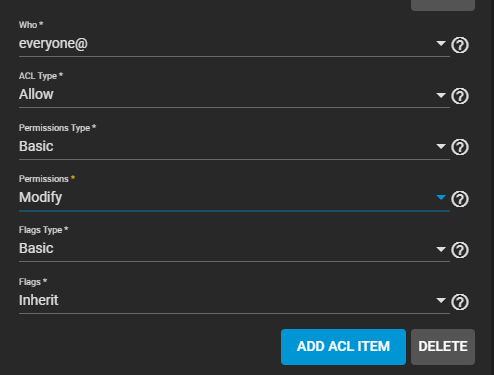
\includegraphics[width=\linewidth]{img/ss_truenas/43.png}
    \caption{Parametry presetu ACL dla wszystkich}
\end{figure}

Po wykonaniu wszystkich czynności możemy przetestować działanie udziału sieciowego w systemie Windows. W tym celu mapujemy dysk sieciowy, podając adres do folderu, którego nazwa to nazwa naszego datasetu. Po zatwierdzeniu danych system zapyta nas o dane logowania użytkownika, który posiada dostęp do tego udziału. Po podaniu prawidłowych danych możemy już korzystać z udziału sieciowego jako zmapowanego dysku.

\begin{figure}[H]
    \centering
    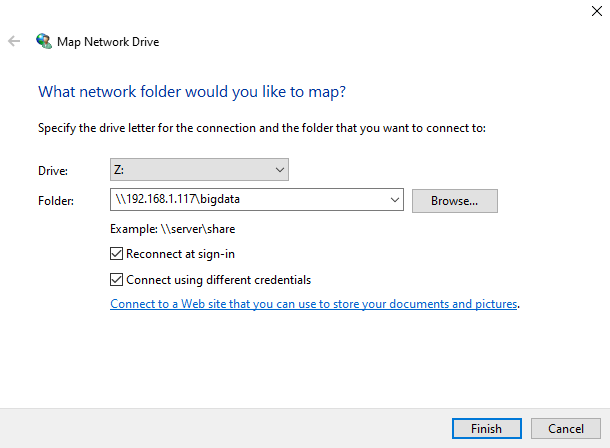
\includegraphics[width=14cm]{img/ss_truenas/45.png}
    \caption{Mapowanie dysku sieciowego w systemie Windows}
\end{figure}

\begin{figure}[H]
    \centering
    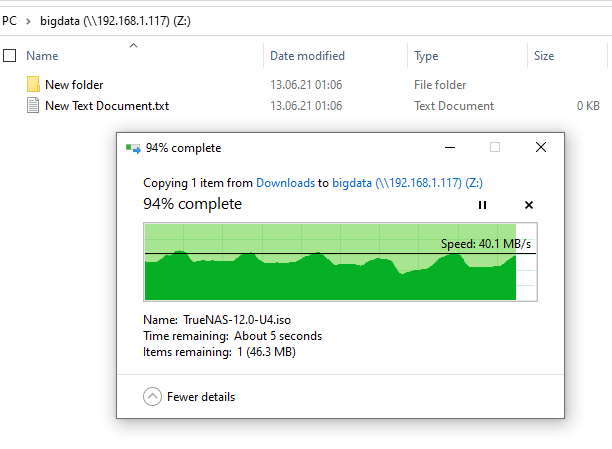
\includegraphics[width=14cm]{img/ss_truenas/50.png}
    \caption{Uzyskanie dostępu do dysku sieciowego oraz tworzenie przykładowych danych}
\end{figure}

\newpage
\subsection{Konfiguracja Plex i DLNA}

Po postawieniu oprogramowania TrueNAS i skonfigurowaniu 4 dysków w RAID5 kolejnym etapem projektu jest postawienie funkcji multimedialnych DLNA. Sam standard DLNA jest już dość stary i generalnie zalecanym rozwiązaniem do multimediów jest oprogramowanie Plex, które jest tak jakby klonem Netflixa dającym dostęp do darmowych produkcji oraz produkcji znajdujących się lokalnie na serwerze. Dodatkowo wspiera udostępnianie lokalnych multimediów po protokole DLNA.

Dodatkowe funkcje w TrueNAS instaluje się pobierając pluginy. Pluginy w TrueNAS działają w tzw. jailach, czyli kontenerach które znajdują się w specjalnie utworzonym datasecie. Dataset ten może znajdować się gdziekolwiek, jednak z powodów szybkości działania warto, aby był na SSD w miarę możliwości. Z tego też powodu do naszej maszyny wirtualnej dodany został kolejny dysk twardy przeznaczony tylko na jaile. Planowo miał być tylko wykorzystywany na instalacje i konfiguracje pluginów, z tego też powodu nie posiada żadnych zabezpieczeń przed awarią (żadnej duplikacji RAID).

\begin{figure}[H]
    \centering
    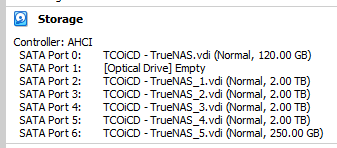
\includegraphics{img/ss_plex/1.png}
    \caption{Dodany nowy dysk SSD do maszyny wirtualnej}
\end{figure}

Po dodaniu nowego dysku, aby móc go wykorzystywać w systemie konieczne jest stworzenie na nim datapoola. TrueNAS z uwagi na swoje zastosowania ostrzega przed tworzeniem pooli nie będących chronionych przed awarią.

\begin{figure}[H]
    \centering
    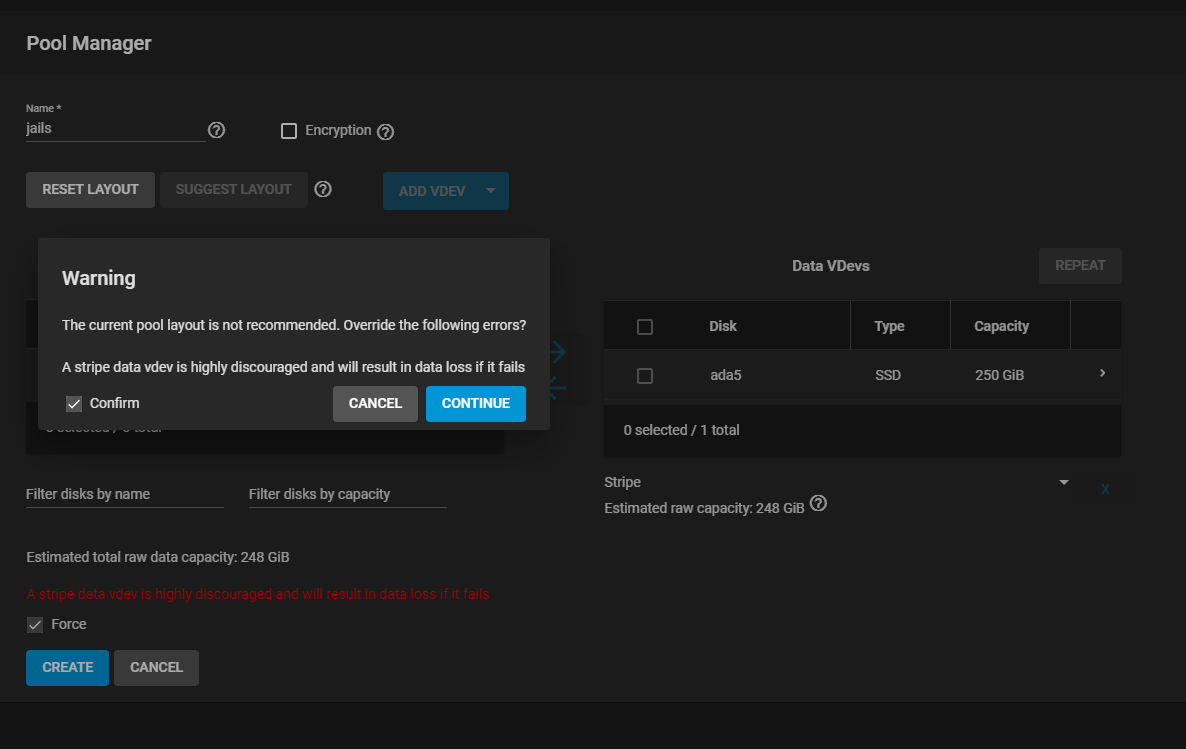
\includegraphics[width=\linewidth]{img/ss_plex/2.png}
    \caption{Tworzenie nowego datapoola na jaile - ostrzeżenie o braku zabezpieczenia przed awarią dysku}
\end{figure}

\begin{figure}[H]
    \centering
    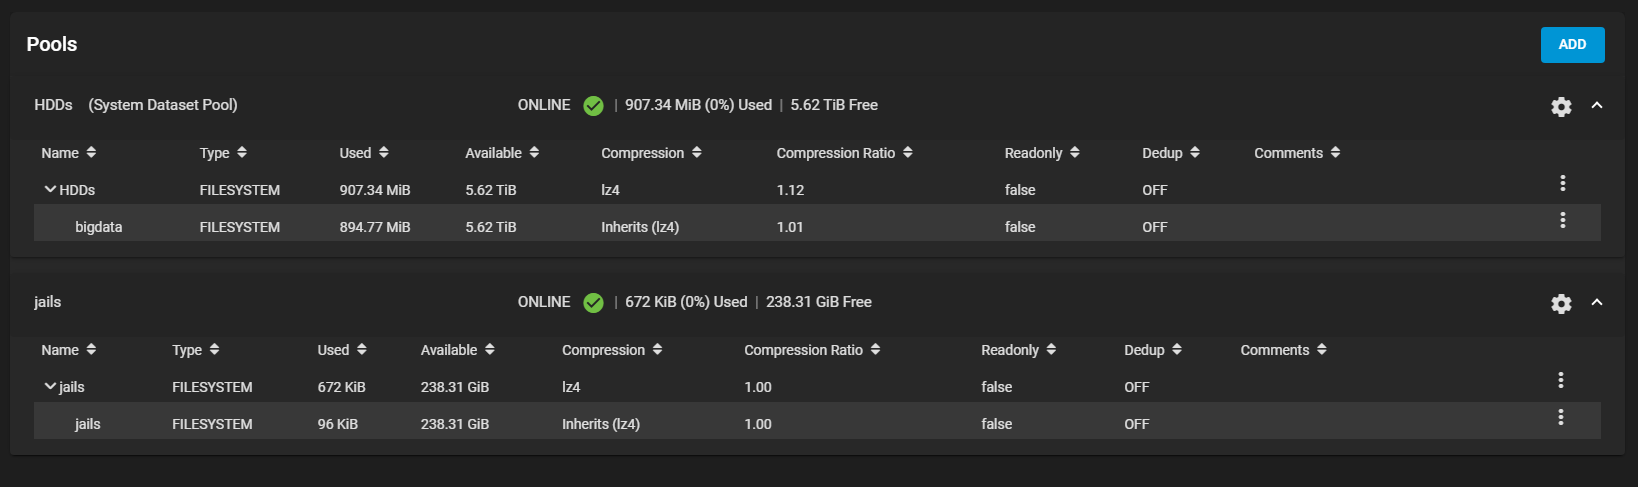
\includegraphics[width=\linewidth]{img/ss_plex/3.png}
    \caption{Wszystkie datapoole i datasety na serwerze}
\end{figure}

Po utworzeniu odpowiednich pooli kolejnym krokiem jest instalacja pluginu. Pierwsze otwarcie zakładki z pluginami skutkuje pytaniem o miejsce przechowywania danych pluginów - w naszym wypadku wybieramy nowo utworzony datapool.

\begin{figure}[H]
    \centering
    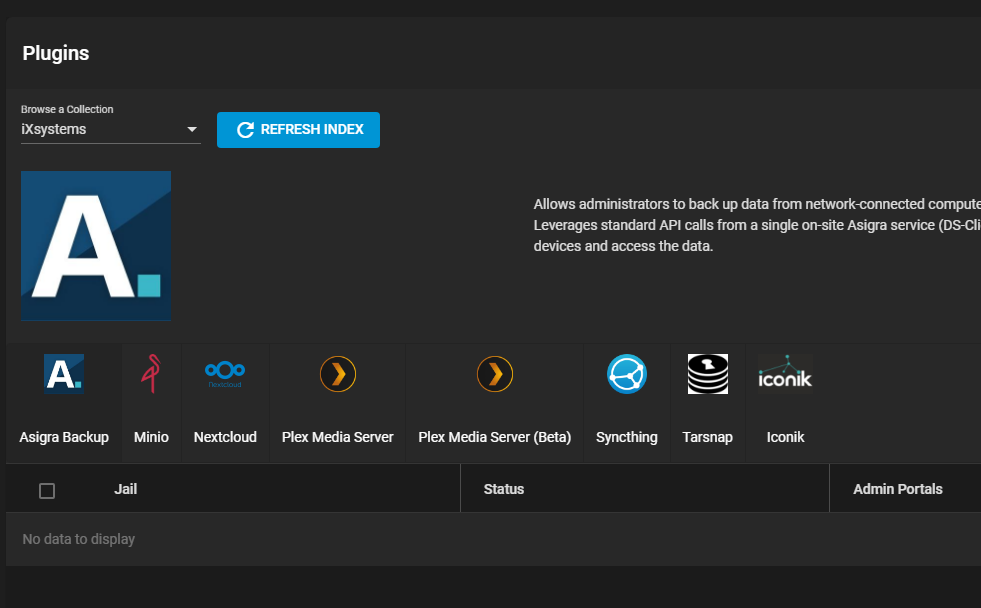
\includegraphics[width=\linewidth]{img/ss_plex/4.png}
    \caption{Oficjalna lista pluginów - poza nimi dostępna jest również bogata baza pluginów społeczności}
\end{figure}

Kolejnym etapem jest wystartowanie instalacji pluginu Plex z domyślnymi ustawieniami. Tutaj niestety z uwagi na problem z wirtualną kartą sieciową wystąpił problem instalacji i konieczne było przestawienie ustawień pluginu na statyczny adres IP. Z takimi ustawieniami plugin poprawnie się zainstalował co widać na poniższym zrzucie ekranu.

\begin{figure}[H]
    \centering
    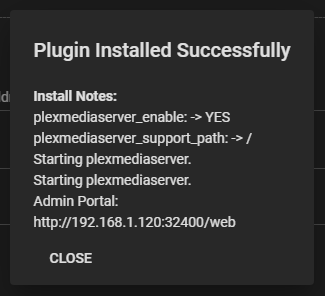
\includegraphics{img/ss_plex/7.png}
    \caption{Poprawna instalacja pluginu Plex}
\end{figure}

Następnym krokiem jest przygotowanie datasetu na multimedia. Warto aby to był osobny dataset, aby nie udostępniam Plexem całości NASa, zwłaszcza jeśli planujemy wystawiać Plex poza swoją sieć lokalną. Tworzymy więc nowy dataset oraz nowego share'a, aby móc podłączyć się do tego datasetu z poziomu Windowsa.

\begin{figure}[H]
    \centering
    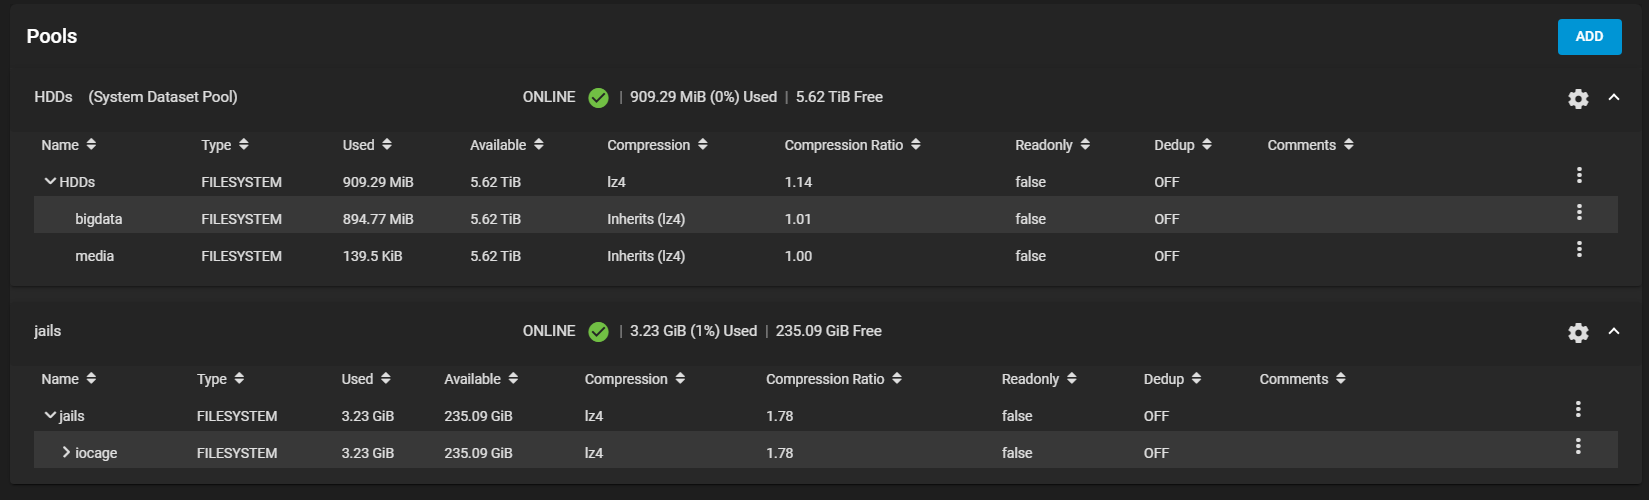
\includegraphics[width=\linewidth]{img/ss_plex/11.png}
    \caption{Utworzone datasety na serwerze}
\end{figure}

\begin{figure}[H]
    \centering
    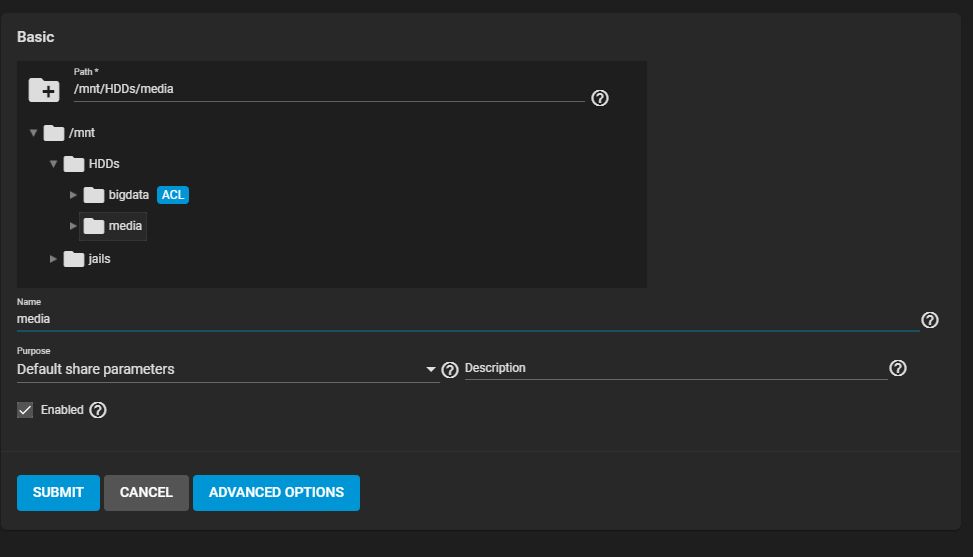
\includegraphics[width=\linewidth]{img/ss_plex/12.png}
    \caption{Tworzenie nowego share'a}
\end{figure}

Następnym krokiem jest podłączenie do Windowsa drugiego zewnętrznego udziału i wgranie przykładowych multimediów. Wszystkie wykorzystane multimedia do tego projektu są na licencji CC.

\begin{figure}[H]
    \centering
    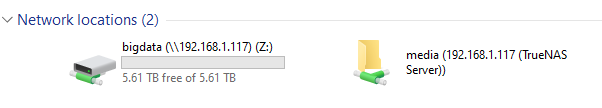
\includegraphics[width=\linewidth]{img/ss_plex/13.png}
    \caption{Zasób media widoczny z poziomu Windowsa}
\end{figure}

\begin{figure}[H]
    \centering
    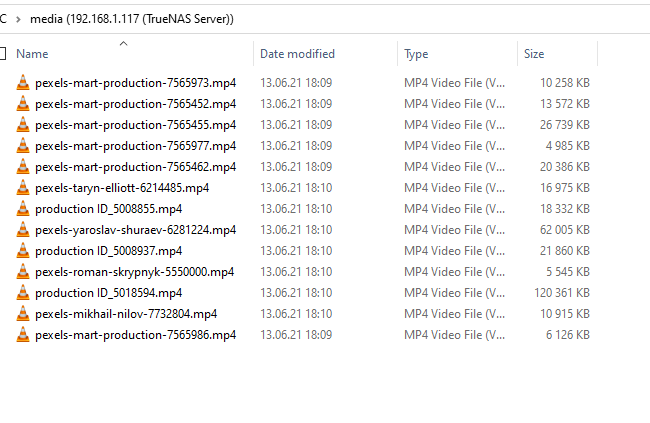
\includegraphics[width=\linewidth]{img/ss_plex/14.png}
    \caption{Lista przykładowych multimediów wgranych na zasób multimediów}
\end{figure}

Następnym krokiem jest zastopowanie usługi Plex i dodanie mountpointa. Mountpoint jest potrzebny aby z poziomu jaila możliwy był dostęp do datasetu poza jailem.

\begin{figure}[H]
    \centering
    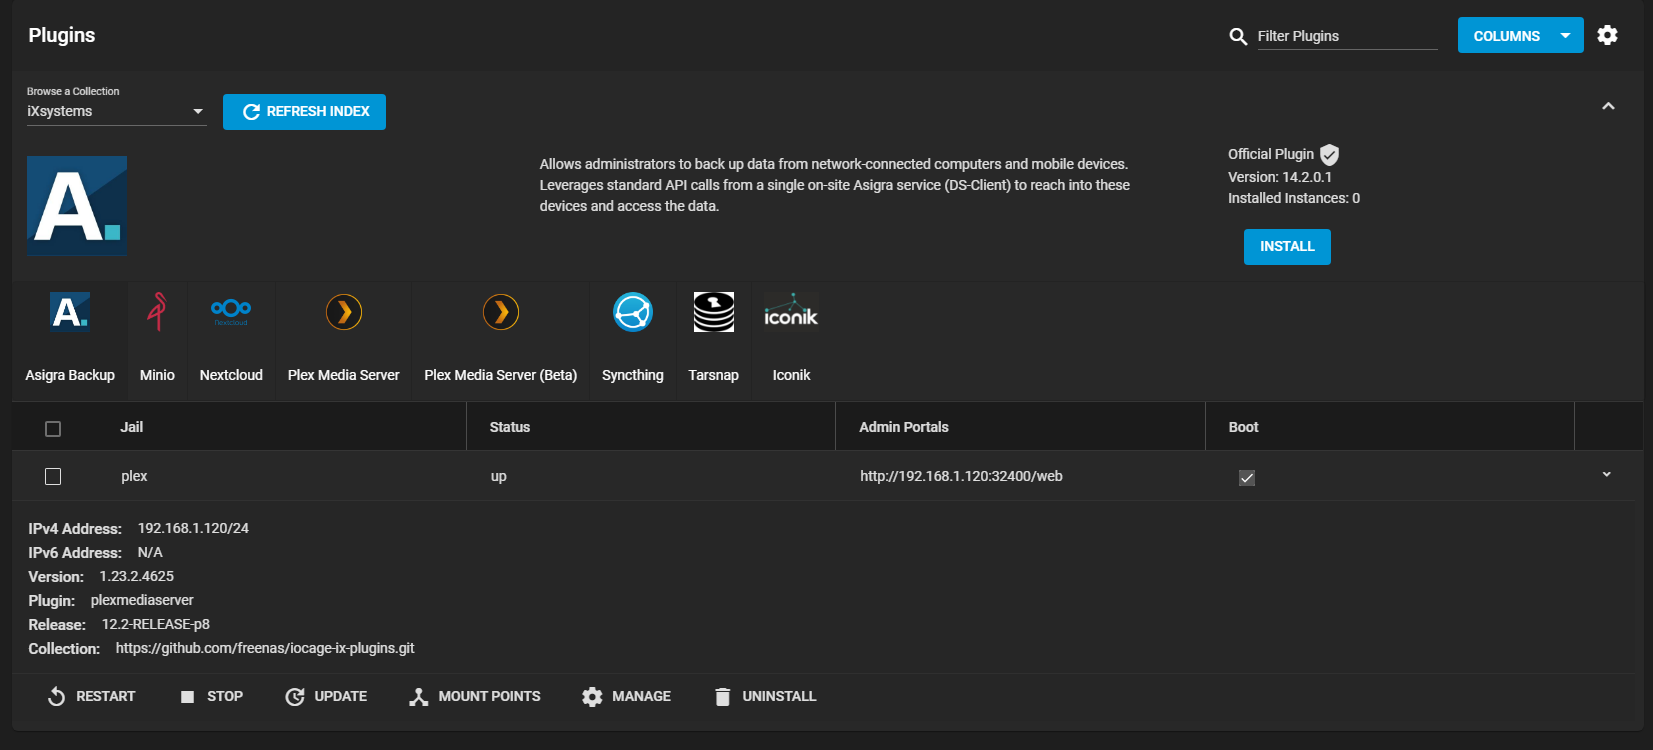
\includegraphics[width=\linewidth]{img/ss_plex/16.png}
    \caption{Szczegóły pluginu Plex}
\end{figure}

\begin{figure}[H]
    \centering
    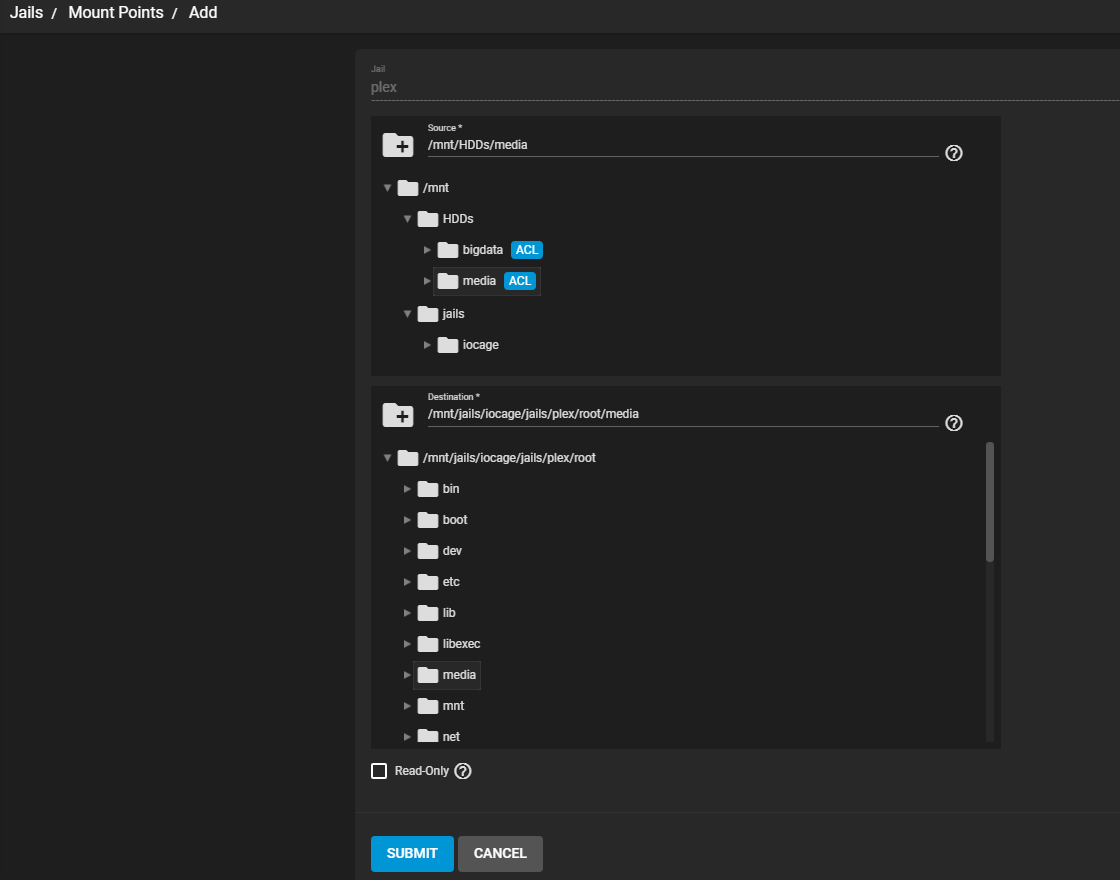
\includegraphics[width=\linewidth]{img/ss_plex/17.png}
    \caption{Dodanie punktu montowania dla jaila}
\end{figure}

Po dodaniu dolinkowania można uruchomić panel zarządzania Plexem. Wita nas tutorial z kilkoma podstawowymi opcjami. Po zakończeniu tutoriala widzimy ekran bardzo zbliżony do ekranu Netflixa zawierający różne darmowe produkcje. W ustawieniach programu dodać można zewnętrzne foldery z multimediami do biblioteki.

\begin{figure}[H]
    \centering
    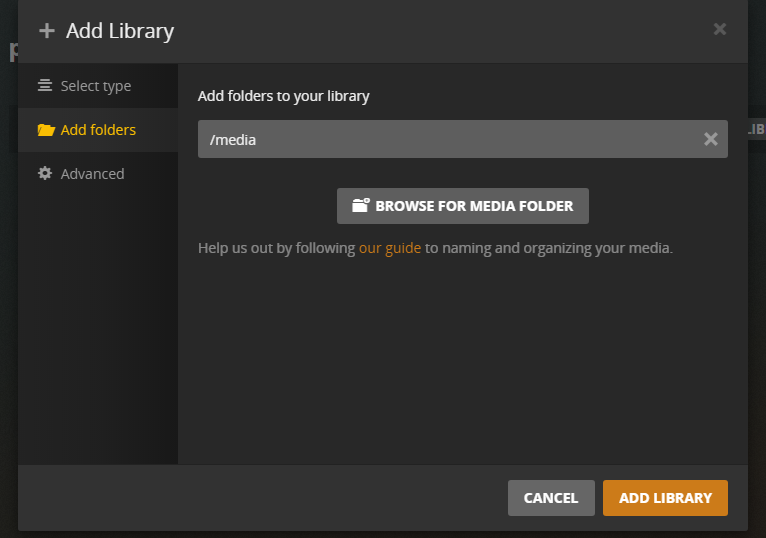
\includegraphics[width=\linewidth]{img/ss_plex/21.png}
    \caption{Dodawanie katalogu z multimediami do biblioteki}
\end{figure}

Po dodaniu nowego folderu na głównym ekranie widzimy nową zakładkę, a w niej dodane wcześniej multimedia.

\begin{figure}[H]
    \centering
    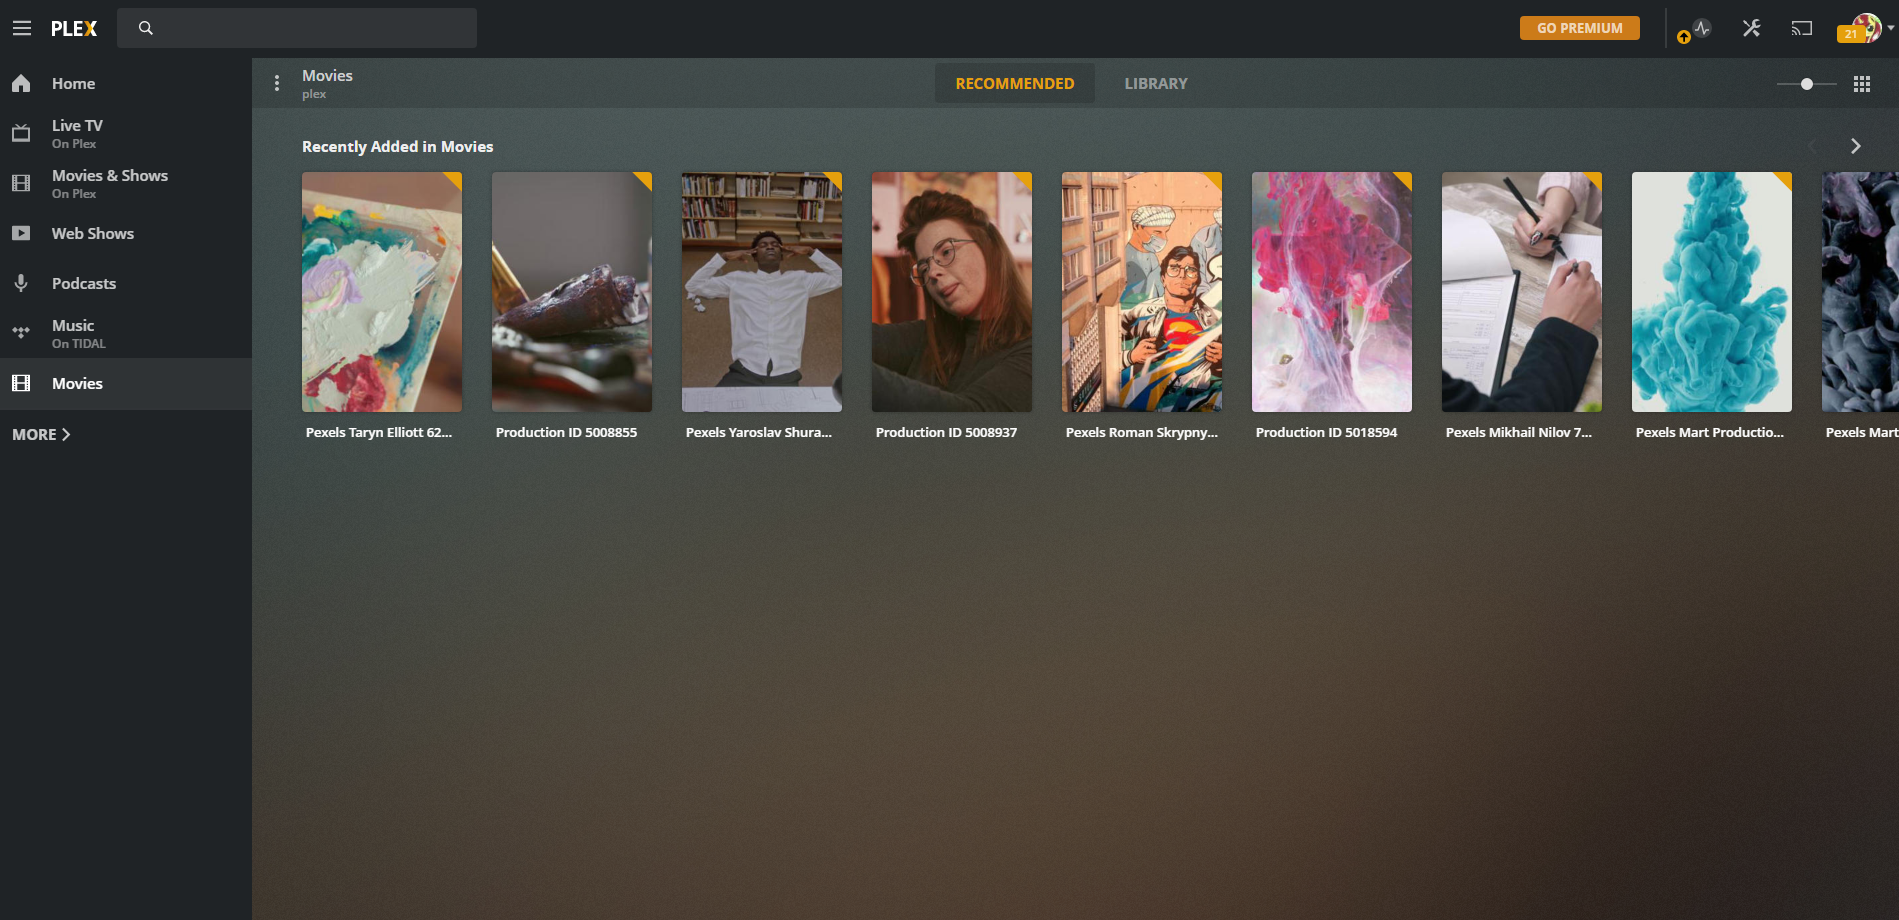
\includegraphics[width=\linewidth]{img/ss_plex/23.png}
    \caption{Widoczne filmy w bibliotece Plexa}
\end{figure}

\begin{figure}[H]
    \centering
    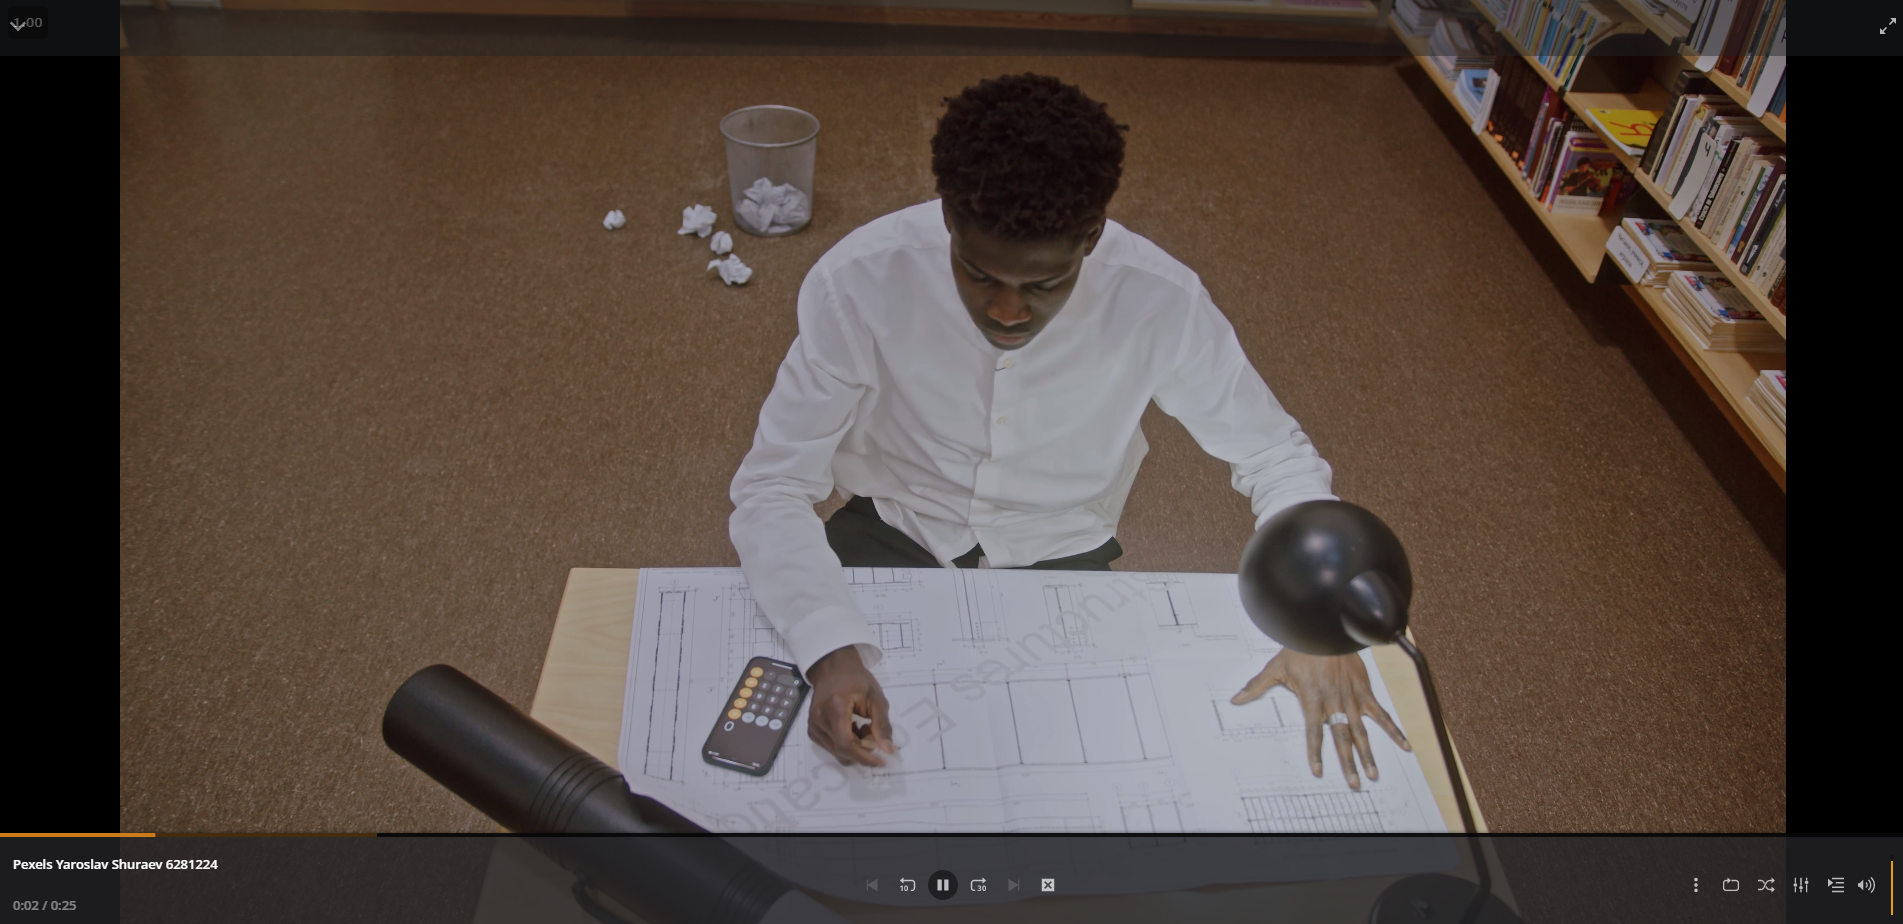
\includegraphics[width=\linewidth]{img/ss_plex/24.png}
    \caption{Odtwarzanie filmu w odtwarzaczu webowym}
\end{figure}

Kolejnym krokiem jest uruchomienie z poziomu ustawień serwera DLNA.

\begin{figure}[H]
    \centering
    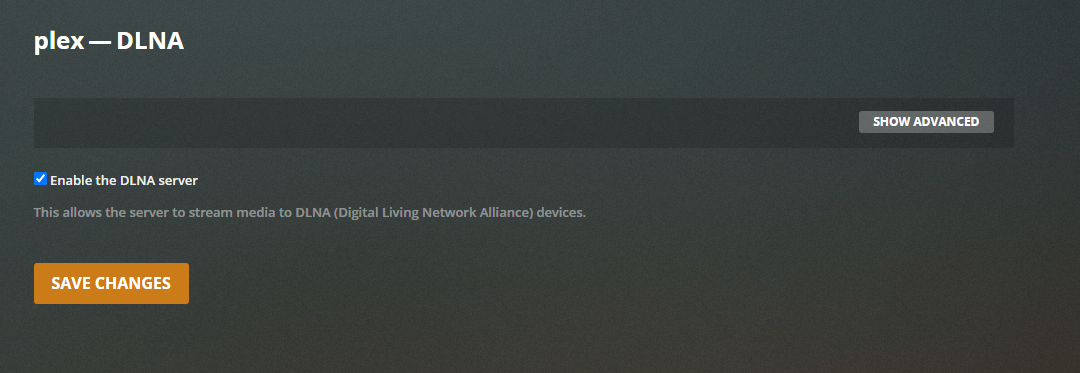
\includegraphics[width=\linewidth]{img/ss_plex/25.png}
    \caption{Uruchomienie usługi DLNA}
\end{figure}

Po uruchomieniu serwera DLNA możemy go zobaczyć z poziomu Windowsa.

\begin{figure}[H]
    \centering
    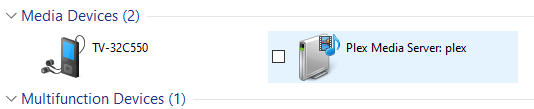
\includegraphics{img/ss_plex/27.png}
    \caption{Widoczny serwer multimedialny Plexa w systemie Windows}
\end{figure}

Dostępny jest on również z poziomu TV.

\begin{figure}[H]
    \centering
    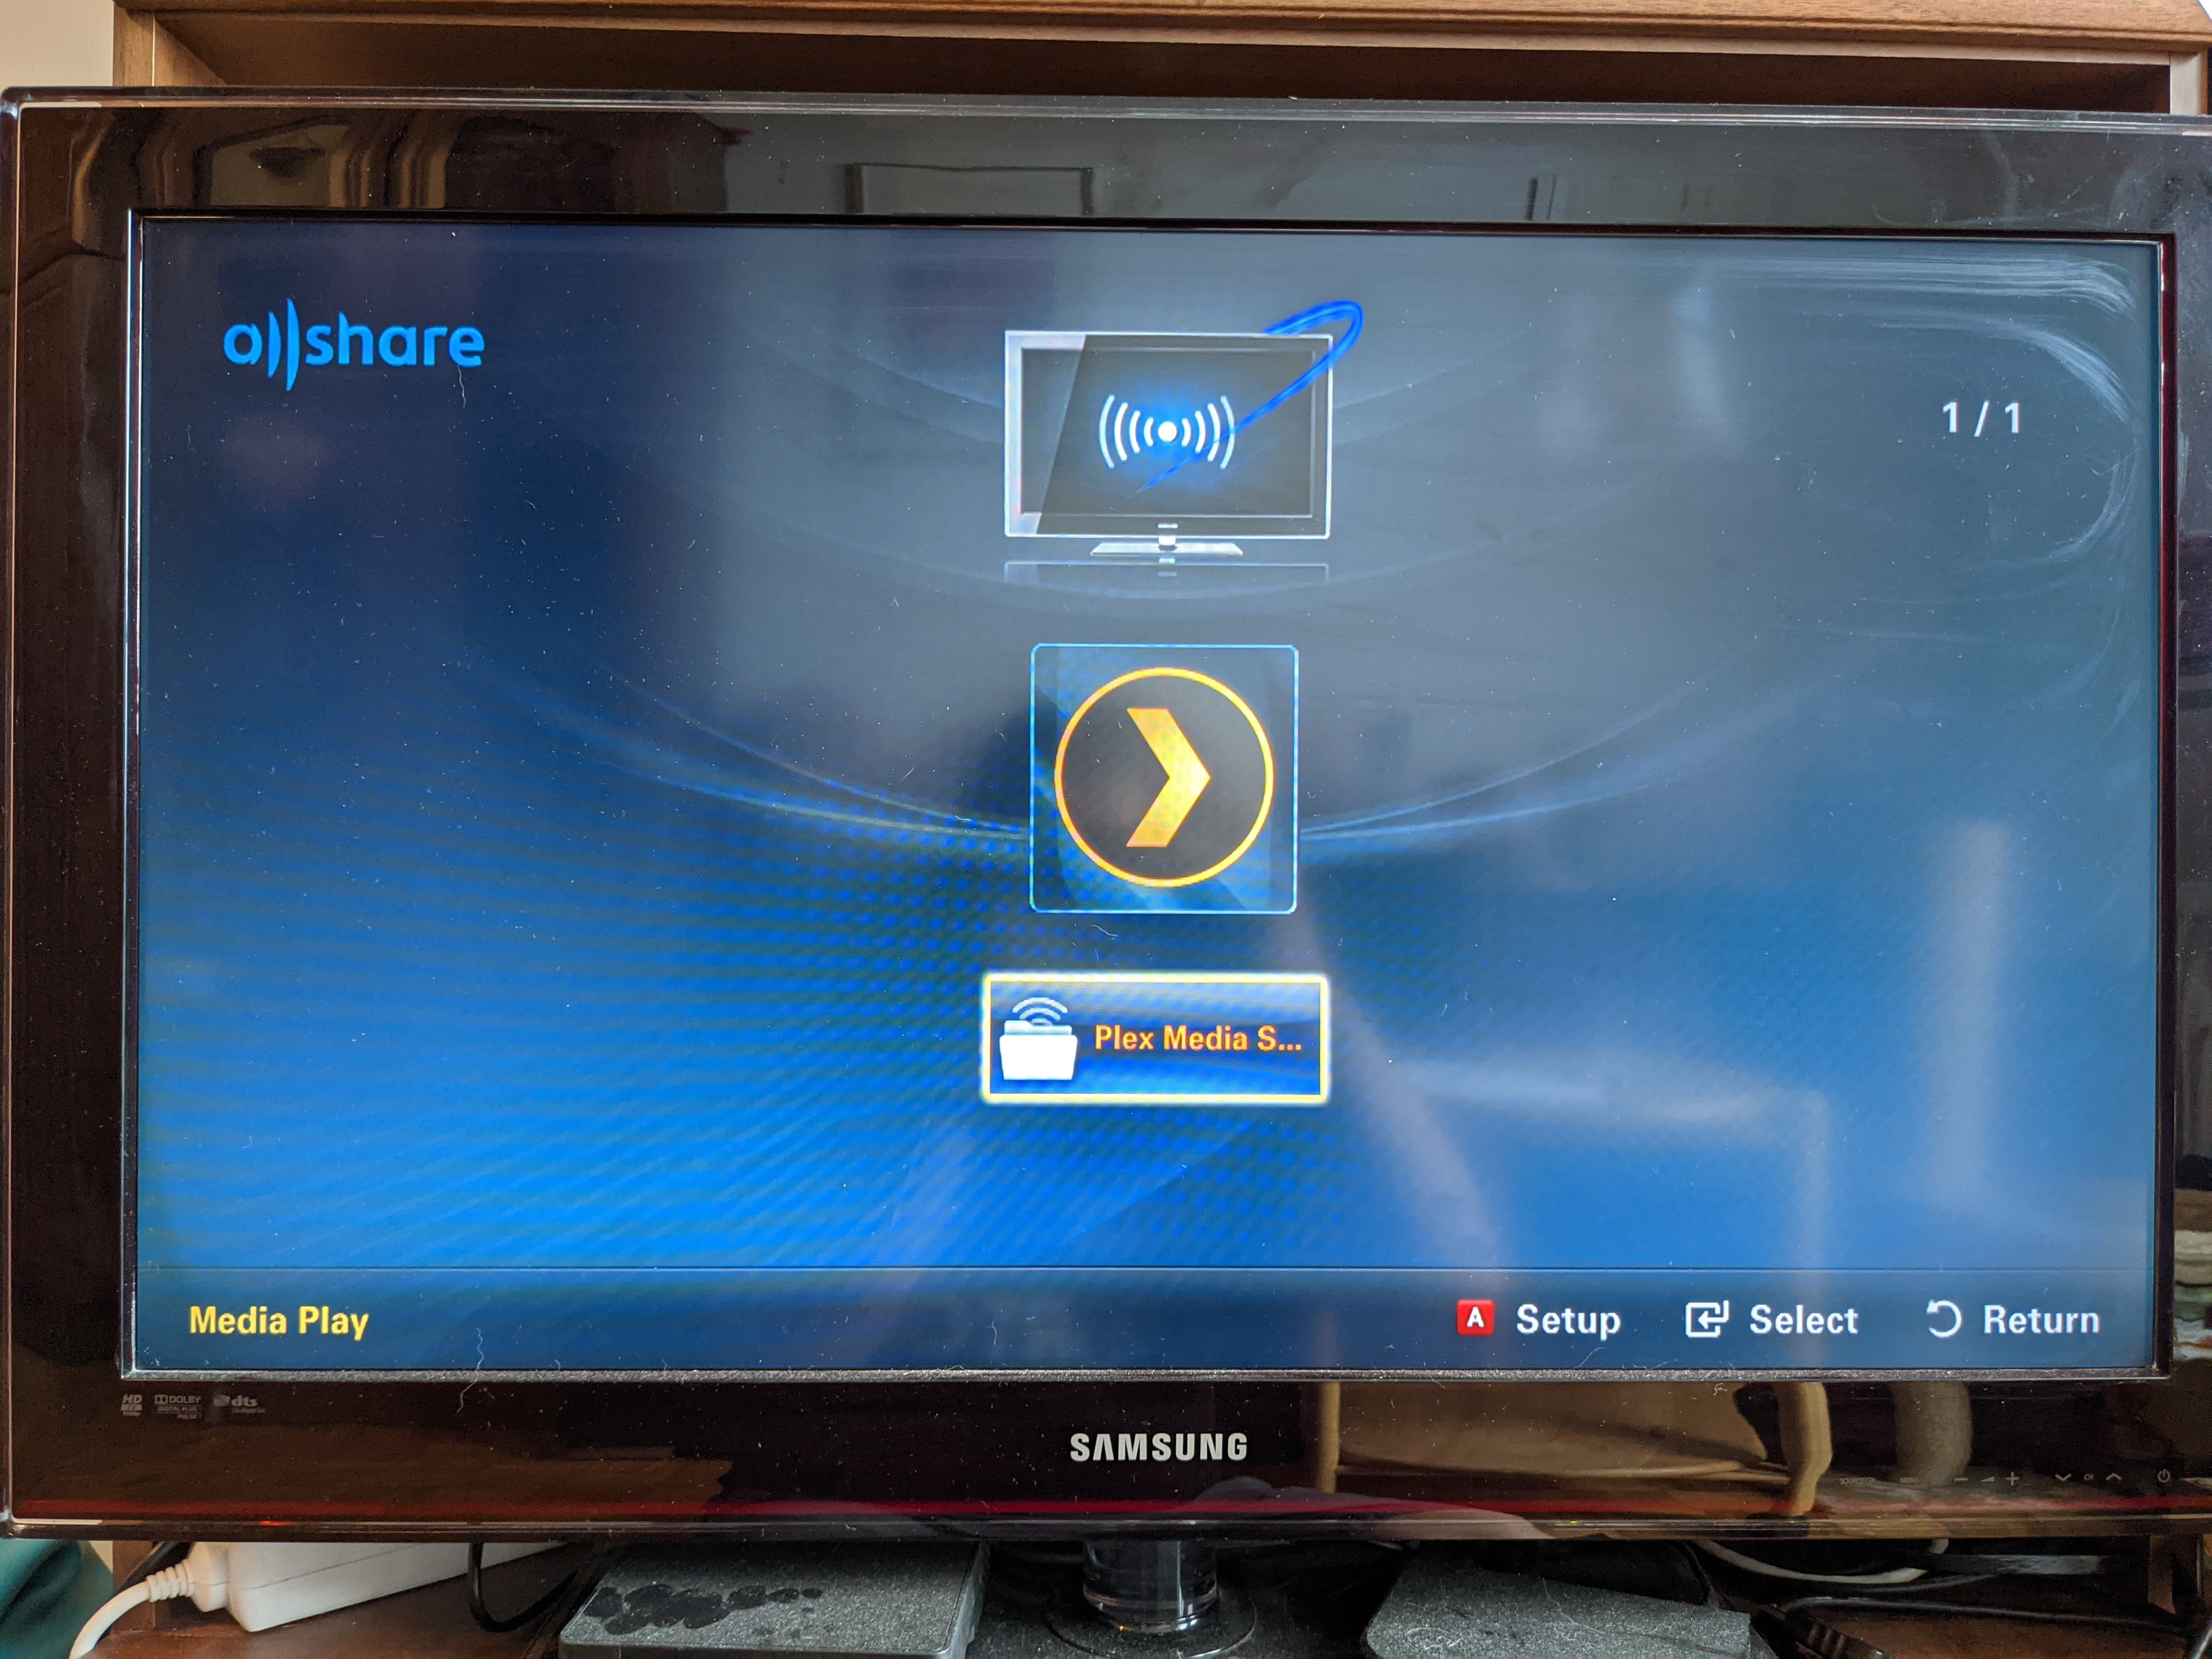
\includegraphics[width=13cm]{img/ss_plex/tv2.jpg}
    \caption{Widoczny serwer multimedialny Plexa na telewizorze}
\end{figure}

\begin{figure}[H]
    \centering
    \includegraphics[width=13cm]{img/ss_plex/tv.jpg}
    \caption{Lista multimediów widoczna na telewizorze}
\end{figure}

W ustawieniach Plexa widzimy również, że dostęp spoza sieci nie jest poprawnie skonfigurowany. Wynika to z braku ustawionego przekierowania portów na routerze. Z tego też powodu niemożliwe jest połączenie się z serwerem Plexa z poziomu mobilnej aplikacji. W tym miejscu przed otworzeniem portu Plexa warto dokończyć konfigurację zabezpieczeń. Jeśli nie planuje się używania Plexa z poza sieci LAN warto wyłączyć remote access. 

\begin{figure}[H]
    \centering
    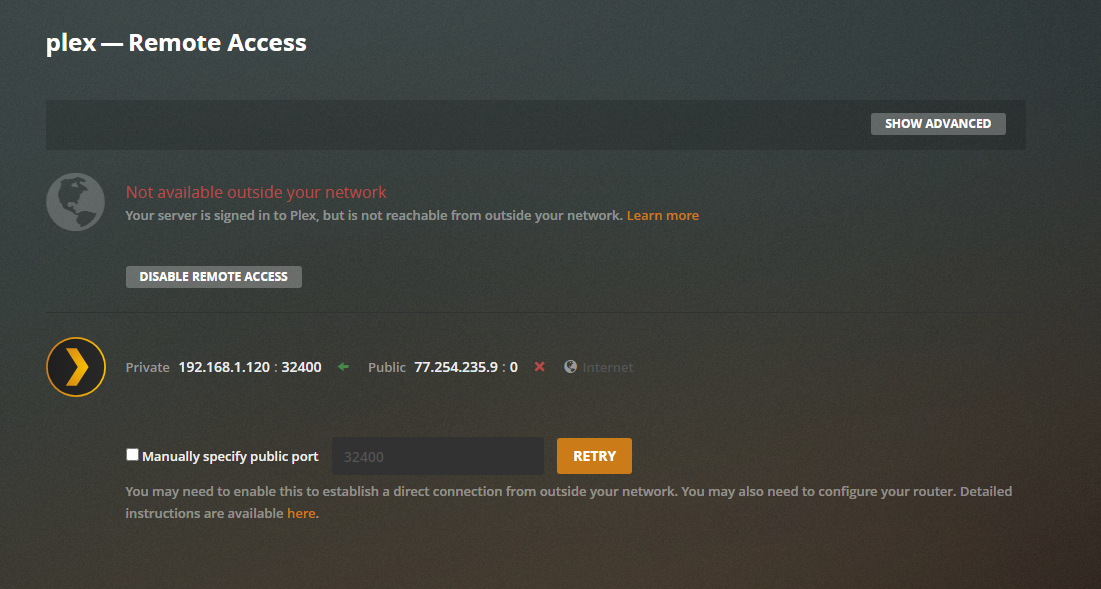
\includegraphics[width=\linewidth]{img/ss_plex/28.png}
    \caption{Ustawianie dostępu zdalnego do Plexa}
\end{figure}


\subsection{Konfiguracja nextCloud}

Kolejnym etapem projektu jest postawienie usługi typu ownCloud, która umożliwia podobną funkcjonalność co komercyjne usługi typu Google Drive, czy Dropbox.

Pierwszym etapem jest zainstalowanie plugina nextCloud (który jest forkiem ownCloud) na serwerze TrueNAS (instalacja polega na wybraniu plugina z biblioteki dostępnych pluginów i uruchomienie procesu instalacji z domyślnymi ustawieniami).

\begin{figure}[H]
    \centering
    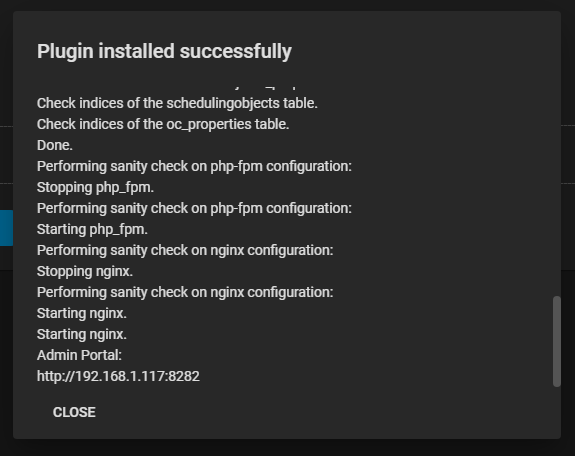
\includegraphics[width=\linewidth]{img/ss_cloud/29.png}
    \caption{Poprawna instalacja plugina nextCloud}
\end{figure}

Plugin został zainstalowany na stworzonym w poprzednim kroku datapoolu \texttt{jails}, a więc pojedynczym dysku SSD, który nie jest w żaden sposób zabezpieczony przed awarią. Podczas, gdy w poprzednim kroku na tym dysku były tylko pliki usługi (właściwe dane znajdowały się na datasecie \texttt{HDDS/media}), tak tutaj jest troszkę inaczej i przy domyślnej konfiguracji pliki użytkowników wgrane do nextCloud będą na tym niezabezpieczonym dysku SSD.

Aby zabezpieczyć dane użytkowników możliwe jest podlinkowanie nowego bądź istniejącego już datasetu do jaila zawierającego nextCloud oraz podmienienie ścieżki, gdzie znajdują się pliki użytkowników. Robiąc to zyskujemy miejsce, jednak tracimy szybkość dysku SSD z domyślnej konfiguracji. Dodatkowo usługa nextCloud jak każda inna tego typu działa w formie synchronizacji, a więc kopia danych użytkowników jest na podłączonych urządzeniach i z niej możliwe jest przywrócenie danych w przypadku awarii dysku SSD (tylko danych użytkownika, nie konfiguracji usługi oczywiście). Większość zastosowań dla takich chmur to przechowywanie małych ilości danych, które ma się wielu urządzeniach, więc rozmiar dysku SSD powinien również być wystarczający. Z tych powodów zdecydowaliśmy, że lepszym rozwiązaniem będzie pozostawienie domyślnej lokalizacji plików nextCloud. Natomiast dostęp do reszty plików znajdujących się na NASie z poziomu nextCloud skonfigurowany został wykorzystając external storages, o czym więcej napiszemy później.

Po instalacji widzimy ekran szczegółów dotyczących zainstalowanego pluginu oraz jaila w którym się znajduje.

\begin{figure}[H]
    \centering
    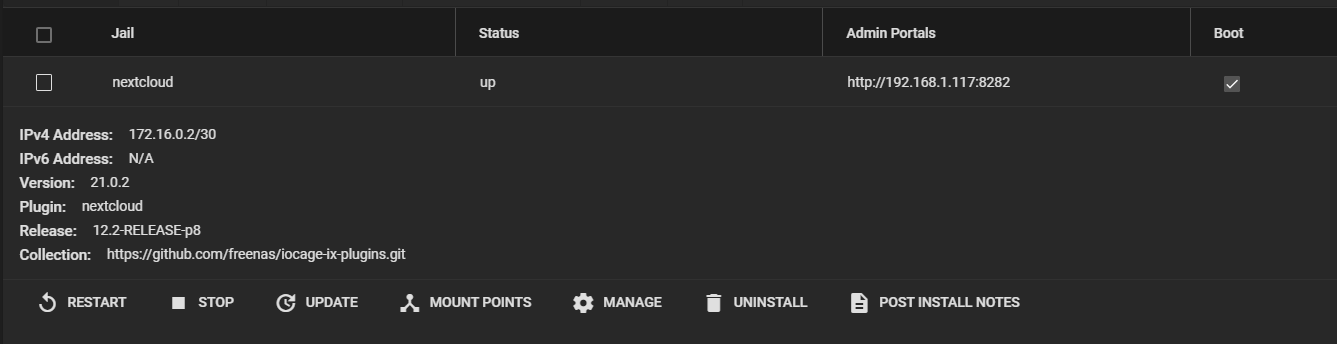
\includegraphics[width=\linewidth]{img/ss_cloud/30.png}
    \caption{Szczegółowe informacje nt. nextCloud}
\end{figure}

Klikając Post Install Notes można sprawdzić hasło do głównego konta administratora usługi nextCloud.

\begin{figure}[H]
    \centering
    \includegraphics[width=13cm]{img/ss_cloud/31.png}
    \caption{Hasło admina nextCloud}
\end{figure}

Po instalacji i zalogowaniu się na admina usługi wita nas ekran podstawowej konfiguracji.

\begin{figure}[H]
    \centering
    \includegraphics[width=\linewidth]{img/ss_cloud/32.png}
    \caption{Ekran powitalny nextCloud}
\end{figure}

Po zakończeniu wprowadzającego tutoriala widzimy, że usługa sama w sobie prawie od razu jest skonfigurowana do jakiegoś działania, następne kroki konfiguracyjne zależą już mocno od tego w jaki sposób chcemy wykorzystywać naszą instancję nextCloud. Na pewno koniecznym krokiem będzie dodanie swojego użytkownika, aby nie logować się w codziennym użytkowaniu na konto admina.

\begin{figure}[H]
    \centering
    \includegraphics[width=\linewidth]{img/ss_cloud/34.png}
    \caption{Utworzenie użytkownika nextCloud}
\end{figure}

Po utworzeniu użytkownika mamy w pewnym sensie działająca instancję nextCloud. Dostęp do niej jest tylko z sieci lokalnej oraz nie ma dostępu do plików z poza głównego katalogu nextClouda. Tak jak wcześniej pisaliśmy dolinkowanie pozostałej zawartości NASa do nextClouda jest możliwe za pomocą mount pointów oraz external storages. Aby to zrobić trzeba zacząć od wyłączenia usługi i dodania mountpointów.

\begin{figure}[H]
    \centering
    \includegraphics[width=\linewidth]{img/ss_cloud/36.png}
    \caption{Dodane mount pointy dla jaila zawierającego nextCloud}
\end{figure}

Po dodaniu mountpointów uruchamiamy ponownie usługę nextCloud i z poziomu konfiguracji tej usługi ustawiamy odpowiednie external storages.

\begin{figure}[H]
    \centering
    \includegraphics[width=\linewidth]{img/ss_cloud/38.png}
    \caption{Ustawienie linków do katalogów zewnętrznych}
\end{figure}

Teraz z poziomu nextCloud mamy dostęp do obu datasetów znajdujących się na macierzy RAID.

\begin{figure}[H]
    \centering
    \includegraphics[width=\linewidth]{img/ss_cloud/40.png}
    \caption{Katalogi zewnętrzne widoczne na poziomie głównego ekranu nextCloud}
\end{figure}

\begin{figure}[H]
    \centering
    \includegraphics[]{img/ss_cloud/41.png}
    \caption{Zawartość datasetu bigdata}
\end{figure}

Oczywiście nie jest to pełna konfiguracja, w dalszym ciągu nie skonfigurowane zostały takie podstawowe aspekty, jak zabezpieczenia, serwer SMTP do poczty do odzyskiwania hasła czy dostęp spoza LANu. Konfiguracja tego jednak jest mocno pracochłonna i wymaga dokonania kilku decyzji. W porównaniu do Plexa nie jest zalecane (nawet po pełnej konfiguracji zabezpieczeń, jak np. SSL) wystawianie portu na zewnątrz LANu do nextClouda, a raczej stworzenie dodatkowego serwera VPN i łączenie się poprzez niego do sieci lokalnej i dalej do nextClouda. Z uwagi na skomplikowanie tego rozwiązania nie konfigurowaliśmy w ramach tego projektu żadnej metody na połączenia spoza LANu.

Natomiast połączenie wewnątrz LANu z poziomu aplikacji mobilnej zostało przetestowane i ukazane na kolejnych zrzutach ekranu.

\begin{figure}[H]
    \centering
    \includegraphics[width=\linewidth]{img/ss_cloud/m7.png}
    \caption{Logowanie do aplikacji mobilnej i wyświetlenie zawartości katalogów}
\end{figure}

\newpage
\section{Podsumowanie}
W ramach niniejszego projektu zrealizowaliśmy szereg czynności, które pozwoliły na utworzenie domowego serwera multimedialnego. Udało się zrealizować nie tylko serwer multimedialny DLNA wraz z chmurą, ale serwer ten posiada także dużo innych funkcjonalności ułatwiających zarządzanie plikami. Serwer działa na oprogramowaniu, które zamienia go w pełnoprawny NAS, który dodatkowo można rozszerzać o dodatkowe funkcje za pomocą bogatej bazy pluginów. 

Aby móc zrealizować funkcję DLNA potrzebowaliśmy pluginu Plex, w którym funkcja udostępniania multimediów za pomocą protokołu DLNA jest funkcją dodatkową. Plex to cyfrowy odtwarzacz multimediów i narzędzie organizacyjne, które umożliwia dostęp do muzyki, zdjęć i filmów przechowywanych na serwerze za pomocą dowolnego innego komputera, dekodera lub zgodnego urządzenia mobilnego. Jego obsługa jest podobna jak obsługa dzisiejszych platform i rozwiązań VOD. Serwer DLNA przetestowaliśmy dodając na niego przykładowe filmy, a następnie je odtwarzając na komputerze oraz na telewizorze. Na obu urządzeniach serwer jest widoczny. Odtwarzanie filmów zadziałało na komputerze, ale na telewizorze nie ze względu na przestarzałe oprogramowanie telewizora, które nie wspiera kodeka H.264.

Do realizacji funkcji chmury z danymi użyliśmy nextCloud, dzięki któremu uzyskaliśmy dostęp do plików znajdujących się na serwerze z poziomu aplikacji webowej oraz mobilnej. Możemy również przesyłać nowe pliki, a także je udostępniać innym użytkownikom.

Projekt okazał się również dla nas pomocny w przyszłym wyborze rozwiązań NAS, które być może zaimplementujemy w swoich domach jako serwer multimediów, a także prosty sposób na współdzielenie plików między użytkownikami w domu oraz prosty system do tworzenia kopii zapasowych. Realizując projekt mieliśmy okazję przetestować rozwiązanie TrueNAS w wirtualnym środowisku, czego najprawdopodobniej nie zrobilibyśmy siadając do tworzenia własnego serwera NAS. Wiedza, którą posiedliśmy w ramach tego projektu zostanie na pewno dobrze spożytkowana.

\newpage
\addcontentsline{toc}{section}{Źródła}
\begin{thebibliography}{}

\bibitem{truenas_download} TrueNAS - Strona producenta
\newline\url{https://www.truenas.com/download-truenas-core/}

\bibitem{filmy_cc} Filmy na licencji Creative Commons
\newline\url{https://www.pexels.com/search/creative%20commons/}


\end{thebibliography}
%\bibliographystyle{unsrt}
%\bibliography{references}
%\listoffigures % WHAT THE ACTUAL FUCK?! WHY IS IT EVEN HERE?!
\end{document}
